\documentclass[12pt]{article}
\usepackage{amsmath, amsfonts, amssymb, amsthm, mathdots, mathrsfs, dsfont,systeme}
\usepackage[utf8]{inputenc}
\usepackage[spanish]{babel}
\usepackage{color}
\usepackage{fancyhdr}
\usepackage{enumerate}
\usepackage{hyperref}
\hypersetup{
    colorlinks=true,
    linkcolor=blue,
    filecolor=magenta,   
    citecolor=blue,
    urlcolor=cyan,
    pdftitle={Algebra lineal},
    pdfpagemode=FullScreen,
    }
\usepackage{amscd}
\usepackage{nomencl}
\usepackage{tikz}
\usepackage{tikz-cd}
\usepackage{amssymb}
\usepackage{blkarray}
\usepackage{multicol}
\usepackage[a4paper,margin=1cm,footskip=.5cm]{geometry}
\usepackage[all]{xy}
\usepackage{pst-node}
\usepackage{subfigure}
%\usepackage[table]{xcolor}
\usepackage{colortbl}
\newcommand{\cN}{\mathcal{N}}
\newcommand{\V}{\mathbb{V}}
\newcommand{\A}{\mathbb{A}}
\newcommand{\M}{\mathcal{M}}
\newcommand{\cH}{\mathcal{H}}
\newcommand{\F}{\mathcal{F}}
\newcommand{\G}{\mathcal{G}}
\newcommand{\cL}{\mathcal{L}}
\newcommand{\cO}{\mathcal{O}}
\DeclareMathOperator{\Hom}{Hom}
\DeclareMathOperator{\Ns}{NS}
\DeclareMathOperator{\im}{im}
\DeclareMathOperator{\Pic}{Pic}
\DeclareMathOperator{\Div}{Div}
\DeclareMathOperator{\Pdiv}{PDiv}
\DeclareMathOperator{\ddiv}{div}
\DeclareMathOperator{\Cl}{Cl}
\DeclareMathOperator{\CaDiv}{CaDiv}
\DeclareMathOperator{\Mor}{Mor}
\DeclareMathOperator{\Spec}{Spec}
\DeclareMathOperator{\id}{id}
\DeclareMathOperator{\Aut}{Aut}
\DeclareMathOperator{\End}{End}
\DeclareMathOperator{\CH}{CH}
\DeclareMathOperator{\IM}{Im}
\DeclareMathOperator{\Pf}{Pf}
\DeclareMathOperator{\Gl}{GL}
\DeclareMathOperator{\Sl}{SL}
\DeclareMathOperator{\St}{St}
\DeclareMathOperator{\tr}{Tr}
\DeclareMathOperator{\Gr}{Gr}
\DeclareMathOperator{\diag}{diag}
\DeclareMathOperator{\ord}{ord}
\DeclareMathOperator{\supp}{supp}
\DeclareMathOperator{\sign}{sign}
\DeclareMathOperator{\adj}{adj}
\DeclareMathOperator{\nul}{nul}
\DeclareMathOperator{\ran}{ran}
\newcommand{\calP}{\cal{P}}
\newcommand{\p}{\mathbb{P}}
\newcommand{\R}{\mathbb{R}}
\newcommand{\Z}{\mathbb{Z}}
\newcommand{\Q}{\mathbb{Q}}
\newcommand{\C}{\mathbb{C}}
\newcommand{\N}{\mathbb{N}}
\newcommand{\bbH}{\mathbb{H}}
\setlength{\parindent}{0pt}
\setlength{\textwidth}{6.5in}
\setlength{\textheight}{9.0in}
\setlength{\topmargin}{0in}
\setlength{\oddsidemargin}{0in}
\newtheoremstyle{exampstyle}
  {\topsep} % Space above
  {\topsep} % Space below
  {\itshape} % Body font
  {} % Indent amount
  {\bfseries} % Theorem head font
  {.} % Punctuation after theorem head
  {.5em} % Space after theorem head
  {} % Theorem head spec (can be left empty, meaning `normal')
\theoremstyle{exampstyle}
\newtheorem{thm}{Teorema}[section]
\newtheorem{prop}[thm]{Proposici\'on}
\newtheorem{lemma}[thm]{Lemma}
\newtheorem{cor}[thm]{Corolario}
\theoremstyle{definition}
\newtheorem{thme}{Expected Theorem}

\newtheorem{rec}[thm]{Recuerdo}
\newtheorem{conj}{Conjecture}
\newtheorem{defin}[thm]{Definici\'on}

\newtheoremstyle{break}%
{}{}%
{}{}%
{\bfseries}{}% % Note that final punctuation is omitted.
{\newline}{}
\theoremstyle{break}
\newtheorem{ejem}[thm]{Ejemplo}
\newtheorem{ejer}[thm]{Ejercicio}
\newtheorem{sol}[thm]{Soluci\'on}
\newtheorem{rmk}[thm]{Observaci\'on}
\numberwithin{equation}{section}
\newcommand{\gb}[1]{\operatorname{\textbf {#1}}}
\hypersetup{linkcolor=black}
% Marca conceptos seleccionados para el índice web de CMSpec.
\newcommand{\cmspecindice}[1]{}
\date{}
\pagestyle{fancy}

\lhead{\includegraphics[width = 4cm]{UFT.png}}
\setlength{\headsep}{0.6in}
\newcolumntype{a}{ >{\columncolor{yellow}} c }

\fancyhead[RO,LE]{
Prof: Camila Muñoz.\\
01/2025}}



\begin{document}
%\maketitle
%\newpage

\begin{minipage}[r]{17cm}
\vspace{5cm}
\hrule
\begin{center}
\vspace{1cm}
{\color{grey}
\Large{\textbf{Apuntes\\ \'Algebra Lineal\\}}
\vspace{0.8cm}
Camila Muñoz}
\vspace{1cm}
\hrule
\end{center}
\title{Apuntes \'Algebra Lineal }
\end{minipage}





\date{}
\pagestyle{fancy}

\lhead{\includegraphics[width = 4cm]{UFT.png}}
\setlength{\headsep}{0.6in}
\newcolumntype{a}{ >{\columncolor{yellow}} c }

\newpage
\tableofcontents
\section{Vectores y matrices.}
Objetivos:
\begin{itemize}
    \item Familiarizarse con los conceptos de vectores y matrices.
    \item Realizar operaciones de suma y multiplicación por escalar.
    \item Estudiar la definición multiplicación entre matrices y vectores.
    \item Realizar operaciones de la multiplicación entre matrices y
vectores.
\end{itemize}

\subsection{Definiciones generales}
Un \textbf{vector fila} de $n$ componentes (entradas) se define como un conjunto ordenado de $n$ números dispuestos de manera horizontal, es decir 
\[x= \left(\begin{array}{ccccc}
   x_1 & x_2 &  \dots&  x_n 
\end{array}\right),\]
donde cada componente $x_i$ pertenece a un conjunto $K$, usualmente $\R$ o $\C$. 
De la misma manera, un \textbf{vector columna} de $n$ componentes es un conjunto ordenado de $n$ números escritos de forma vertical
\[ x=\left(\begin{array}{c}
   x_1 \\
   x_2 \\
   \vdots\\
   x_n 
\end{array}\right).\]
En ambos casos, si un vector tiene $n$ componentes, se dice que el vector es de dimensión $n$.
\begin{defin}
Una \textbf{matriz $A$ de $m \times n$} es un arreglo rectangular de $mn$ elementos de un conjunto dispuestos en $m$ filas y $n$ columnas:
\[A=\left(\begin{array}{cccccc}
     a_{11}& a_{12} & \dots & a_{1j} &\dots & a_{1n}\\
     a_{21}& a_{22} & \dots &a_{2j} &\dots & a_{2n}\\
     \vdots&  \vdots & \ddots &  \vdots &\ddots &  \vdots\\
     a_{i1}& a_{i2} & \dots &a_{ij} &\dots & a_{in}\\
     \vdots&  \vdots & \ddots & \vdots &\ddots &  \vdots\\
     a_{m1}& a_{m2} & \dots & a_{mj} &\dots & a_{mn}
\end{array}\right)_{m\times n}.\]





De forma abreviada, la matriz $A$ puede denotarse por $A=(a_{ij})$, con $i=1,2,\dots, m$, $j=1,2,\dots, n$, donde el elemento $a_{ij}$ corresponde al número que aparece en la fila $i$ y la columna $j$ de la matriz $A$.

Las matrices usualmente se denotan por letras mayúsculas $A, B,$ etc. y sus respectivas entradas se denotan por la minúscula respectiva $a_{ij}, b_{ij}$, etc.

Si $m =n$ se dice \textbf{matriz cuadrada} y en caso contrario se dice que la matriz es \textbf{rect\'angular}.

El conjunto de matrices de $m\times n$ con entradas en el cuerpo $K$ se denota por $\M_{m\times n}(K)$, en otras palabras
\[\M_{m\times n}(K):=\Big\{A=(a_{ij}) \colon a_{ij}\in K \text{ con $i=1,2,\dots, m$ y $j=1,2,\dots, n$}\Big\}.\]
\end{defin}
En el caso de matrices cuadradas de orden $n$ es escribe $\M_n(K)$.


Una matriz $A$ de $m \times n$ cuyas entradas son todas  iguales a 0, se denomina \textbf{matriz cero} de $m \times n$ y se denota por $0_{m\times n}$.

La matriz cuadrada $I_n=(a_{ij})$ de $n\times n$ tal que 
\[a_{ij}=\left\{\begin{array}{ll}
    1 & \text{ si } i= j, \\
   0 & \text{ si no},
\end{array}\right.\]
se llama \textbf{matriz identidad} de orden $n$. Su nombre se debe a sus propiedades aritm\'eticas, que discutiremos m\'as adelante.

Dos matrices $A=(a_{ij})$ y $B=(b_{ij})$ son iguales si son del mismo tamaño y las componentes correspondientes son iguales, es decir, $a_{ij}=b_{ij}$ para cada $i$ y para cada $j$.

Si $A = (a_{i j})$ es una matriz de orden $m \times n$, la \textbf{transpuesta} de $A$, denotada por $A^t$,
es la matriz de orden $n \times m$ que se obtiene al intercambiar las filas por las columnas
de $A$. En consecuencia, 
\[A^t := (a_{j i }).\]

\begin{ejem}
\begin{enumerate}[(a)]
    \item Un vector fila de dimensi\'on $n$ es una matriz de $1\times n$.
    \item Un vector columna de dimensi\'on $n$ es una matriz de $n\times 1$.
    \item $A=\left(\begin{array}{cc}{} 1 & 2\\ 3 & 4 \end{array}\right)$ es una matriz cuadrada de $2\times 2$.
    \item Las matrices $\begin{pmatrix}1& 6& 2 \\0&3&4\end{pmatrix}_{2\times 3}$ y $\left(\begin{array}{cc}
   1& 0 \\
    6&3\\
    2& 4
\end{array}\right)_{3\times 2}$ son distintas.
    \item La matriz $\begin{pmatrix}
   0& 0& 0& 0 \\
   0&0&0& 0
\end{pmatrix}_{2\times 4}$ es la matriz cero de orden $2\times 4$.
\end{enumerate}
\end{ejem}

\begin{ejer}
\begin{enumerate}[(a)]
    \item Determine la matriz de $4\times 3$ tal que $a_{ij}=i-j$.
    \item De un ejemplo de una matriz $A=(a_{ij})$ tal que $a_{ij}=a_{ji}$ para todo $i$ y para todo $j$.
    \item ?`Existe alguna relaci\'on entre $\M_{1\times n}(\R)$ y $\R^n$?
    \item Construya la matriz $A = (a_{ij})$ de $3 \times 4$, donde
\[a_{ij}=\left\{\begin{array}{ll}
    i & \text{ si } i\leq j, \\
    i+j & \text{ si } i>j
\end{array}\right.\]
\item Encuentre los n\'umeros reales $x,y,z,u,v$ y $w$ tales que se cumple la igualdad
\[\begin{pmatrix}
   -1& x& x-y \\
  u&3&-1
\end{pmatrix}=\begin{pmatrix}
   z& 4& 7 \\
  2&x+v&u+w
\end{pmatrix}\]
Respuesta: $x = 4, y = -3, z = -1, u = 2, v = -1, w = -3$.
\end{enumerate}
\end{ejer}

\begin{rmk}\textbf{?`Por qu\'e estudiar matrices?}

Por su simplicidad y sus propiedades algebraicas, las matrices pueden utilizarse en diversas situaciones, como ordenar datos o representar situaciones pr\'acticas.

La producción semanal, en cientos, de los artículos $p_1$, $p_2$,\dots ,$p_{60}$ que se fabrican en una industria se pueden expresar mediante una matriz $P$ de 60 filas - donde se escribirán los productos elaborados - y 5 columnas que indicarán los días de la semana de lunes a viernes:
\[
P=\begin{blockarray}{cccccc}
    Lu & Ma & Mi &Ju & Vi \\
\begin{block}{(ccccc)c}
 2& 3,5 & 3 &3,2  & 3 & p_1 \\
  6 & 6,5 & 6,3 & 6,2 & 6 & p_2 \\
  \vdots & \vdots & \vdots & \vdots & \vdots & \vdots \\
  4 & 3,8 & 3,5 & 4 & 3,2 & p_{60} \\
\end{block}
\end{blockarray}
 \]
\end{rmk}

\begin{defin}
La \textbf{diagonal de una matriz} $A$ son las entradas $a_{i j}$, tales que $i=j$ y se denota por $\diag(A):=(a_{11}, \dots, a_{nn})$.

Para una matriz cuadrada de orden $n$, se define la \textbf{traza de $A$} como
\[\tr(A):=\sum_{i=1}^{n} a_{ii},\]
es decir, la traza corresponde a la suma de los elementos de la diagonal de una matriz.

Mientras que para un vector $(a_{1} ,a_{2} ,  \dots  a_{n})$ se define \textbf{la matriz diagonal} a la matriz cuadrada
\[\diag(a_{1} ,a_{2} ,  \dots  a_{n}):=\left\{\begin{array}{ll}
    a_i & \text{ si } i=j,\\
    0 & \text{ si no.}
\end{array}\right.\]
\end{defin}


\begin{ejem}
\begin{enumerate}
    \item     $A=\begin{pmatrix}
    2 & 0 & 0\\
    0 & -5 & 0\\
    0 & 0 & 1\\
    \end{pmatrix}
    $ y $B=\begin{pmatrix}
    -1 & 0 \\
    0 & 0 \\
    \end{pmatrix}$ son matrices diagonales.
    \item Para $n\in \N$ se tiene que $\tr(I_n)=n$.
\end{enumerate}

\end{ejem}


\begin{defin}
Una matriz cuadrada $A = (a_{i j})$ se llama \textbf{triangular
superior} si $a_{i j} = 0$ para $i > j$, y se llama \textbf{triangular inferior}
si $a_{i j} = 0$ para $i < j$.

\end{defin}

\begin{ejem}
    $C=\begin{pmatrix}
    4 & -1 & 5\\
    0 & -6 & 0\\
    0 & 0 & 8\\
    \end{pmatrix}
    $ y $D=\begin{pmatrix}
    -3 & 0 \\
    2 & 7 \\
    \end{pmatrix}$ son matrices triangulares superior e inferior respectivamente.
\end{ejem}

\begin{ejem}
    \begin{enumerate}[(a)]
        \item Determine por extensi\'on la matriz $A=(a_{ij})$ de orden 3 dada por
        \[a_{ij}=\begin{cases}
			i, & \text{si $i=j$,}\\
            2i-j, & \text{si $i<j$},\\
            |i-3j| & \text{si $i>j$}.
		 \end{cases}\]
		 \item ¿Cuál es la diagonal y la traza de $A$?
        \item ¿Si la matriz $A$ fuese de orden 20? ¿y si fuese de orden $n$?
    \end{enumerate}
\end{ejem}
% \begin{sol}
% \begin{enumerate}[(a)]
%     \item Directo de la definici\'on se tiene que la matriz 
%     \[A=\begin{pmatrix}
%     a_{11} & a_{12} & a_{13}\\
%     a_{21} & a_{22} & a_{23}\\
%     a_{31}& a_{32} & a_{33}\\
%     \end{pmatrix}=\begin{pmatrix}
%     1 & 0 & -1\\
%     1 & 2 & 1\\
%     0& 3 & 3\\
%     \end{pmatrix},\]
% luego su diagonal es $\diag(A)=(1,2,3)$ mientras que $\tr(A)=6$.  
% \item  Si $A$ es de orden 20 entonces $\tr(A) =\sum_{i=1}^{20} a_{ii}=\sum_{i=1}^{20} i=210$

% \item Si la matriz es de orden $n$, tenemos que $\tr(A) =\sum_{i=1}^{n} a_{ii}=\sum_{i=1}^{n} i=\dfrac{n(n+1)}{2}.$
% \end{enumerate}
% \end{sol}
\begin{defin}
Sea $A = (a_{i j})$ matriz cuadrada. Se dice que $A$ es una matriz \textbf{simétrica} si
$A^t = A$ y se dice que $A$ es \textbf{antisimétrica} si $A^t = -A$, donde $-A$ es la matriz
$-A = (-a_{i j})$.
\end{defin}

\begin{ejem}
    La matriz $A=\begin{pmatrix}
    6 & -1 & 4\\
    -1 & 7 & 2\\
    4& 2 & -3\\
    \end{pmatrix}$ es una matriz simétrica.
\end{ejem}
\begin{ejer}
\begin{enumerate}[(a)]
\item Construya una matriz antisimétrica de orden 4.
\item Si $A$ es una matriz de orden $n$ antisimétrica, demuestre que $ \diag(A)=(0,...,0)$ y que
$\tr(A)=0$. 
\end{enumerate}
\end{ejer}

\begin{ejer}
¿Cuál es la transpuesta de la matriz $A = (a_{ij})$ de orden $3 \times 2$ definida por $a_{i j} = 3i-j^2?$
\end{ejer}

\begin{prop}\label{traspuesta}
$(A^t)^t=A$ para toda $A\in M_{m\times n}(K)$.
\end{prop}
\proof (Ejercicio)



\subsection{Adici\'on y multiplicaci\'on de matrices por un escalar.}
En el conjunto de matrices $M_{m\times n}(K)$ es posible definir dos operaciones:
\begin{defin}
Sean $A = (a_{ij})$ y $B = (b_{ij})$ dos matrices de $m \times n$. Entonces la suma
de $A$ y $B$ es la matriz de $m \times n$
\[A+B=(c_{ij}):=\left(\begin{array}{ccccc}
     a_{11}+b_{11} & \dots & a_{1j}+b_{1j} &\dots & a_{1n}+b_{1n}\\
     a_{21}+b_{21} & \dots &a_{2j}+b_{2j} &\dots & a_{2n}+b_{2n}\\
     \vdots&  \vdots & \ddots &  \vdots &\vdots \\
     a_{m1}+b_{m1} & \dots & a_{mj}+b_{mj} &\dots & a_{mn}+b_{mn}
\end{array}\right)_{m\times n},\]
es decir, $c_{ij}=a_{ij}+b_{ij}$ para cada $i,j$.
\end{defin}

\begin{ejem}
\begin{align*}
    \begin{pmatrix} 1 & 4 & 0 \\ -2 & 6 & 5 \end{pmatrix} + \begin{pmatrix} -3 & 1 & -1 \\ 3 & 0 & 2 \end{pmatrix} &= \begin{pmatrix} 1-3 & 4+1 & 0 -1 \\ -2+3 & 6 + 0 & 5+2 \end{pmatrix}\\
&= \begin{pmatrix} -2 & 5 & -1 \\ 1 & 6 & 7 \end{pmatrix}
\end{align*}
\end{ejem}

\begin{rmk}
La suma $\begin{pmatrix} 1 & 4 & 0 \\ -2 & 6 & 5 \end{pmatrix} + \begin{pmatrix} 4 & 3 \\ 2 & 1 \end{pmatrix} $ 
\\\
no está definida pues las matrices son de distinto tamaño.
\end{rmk}

\begin{defin}
Sea $G$ un conjunto con una operaci\'on (binaria)
\begin{align*}
* \colon G\times G &\to G \\
(a,b) &\mapsto a*b
\end{align*}
diremos que $(G,*)$ es un grupo conmutativo(abeliano), si satisface los siguientes \textit{axiomas}:
\begin{enumerate}
    \item Asociatividad: $(a*b)*c=a*(b*c)$ para todo $a,b,c\in G$.
    \item Elemento neutro: Existe un (\'unico) elemento $e\in G$ tal que para todo $a\in G$ se tiene que $e*a=a*e=a$. Dicho elemento se llama \textbf{elemento neutro del grupo $G$}.
    \item Inverso: Para cada $a\in G$ existe un (\'unico) elemento $b\in G$ tal que $a*b=b*a=e$, donde $e$ es la identidad del grupo. Para cada $a$ el elemento que cumpla la propiedad se llama \textbf{inverso de $a$}.
    \item Conmutatividad: $a*b=b*a$ para todo $a,b\in G$.
\end{enumerate}
\end{defin}

\begin{thm}
El conjunto $\M_{m\times n}(K)$ dotado de la operaci\'on suma, es un grupo abeliano, cuyo elemento neutro es $0_{m\times n}$ y el elemento inverso de una matriz $A=(a_{ij})$ es $-A=(-a_{ij})$
\end{thm}

Se define $A - B := A + (-B)$, para todo $ A, B \in \M_{m\times n}(K)$.

\begin{thm}
Se tiene las siguientes propiedades:
\begin{enumerate}
    \item $\tr(A+B) = \tr(A) + \tr(B)$, para todo $ A, B \in \M_{m\times n}(K)$.
    \item $(A + B)^t = A^t + B^t$, para todo $ A, B \in \M_{m\times n}(K)$.
    \item $A, B$ diagonales, entonces $A + B$ es diagonal.
    \item $A, B$ simétricas, entonces $A + B$ es simétrica.
    \item $A, B$ antisimétricas, entonces $A + B$ es antisimétrica.
    \item $- ( -A) = A$, para toda $ A \in \M_{m\times n}(K)$.
    \item $-(A + B) = -A + (-B)$, para todo $ A, B \in \M_{m\times n}(K)$.
    \item $ A + C = B + C$, entonces  $A = B$.
    \item $ A + X = B$, entonces $X = B - A$.
\end{enumerate}
\end{thm}
\proof (Ejercicio)


\begin{defin}
Si $A$ es una matriz de $m \times n$ y si $\alpha$ es un escalar, es decir un elemento cualquiera del conjunto $K$, entonces la matriz $\alpha \cdot A$ está dada por
\[\alpha \cdot A:=(\alpha \cdot a_{ij})\left(\begin{array}{ccccc}
     \alpha a_{11} & \dots &\alpha  a_{1j} &\dots &\alpha  a_{1n}\\
     \alpha a_{21} & \dots &\alpha  a_{2j} &\dots &\alpha  a_{2n}\\
     \vdots&  \vdots & \ddots &  \vdots &\vdots \\
     \alpha a_{m1} & \dots &\alpha  a_{mj} &\dots &\alpha  a_{mn}
\end{array}\right)_{m\times n}.\]
En general omitiremos el punto ($\cdot$), escribiendo $\alpha A$ en vez de $\alpha \cdot A$.
\end{defin}

\begin{ejem}
    $3\begin{pmatrix}
    2 & -1 & 4\\
    -1 & 5 & 2\\
    \end{pmatrix}=\begin{pmatrix}
    6 & -3 & 12\\
    -3 & 15 & 6\\
    \end{pmatrix}$
\end{ejem}

Con esta definici\'on, es posible mostrar que: 

\begin{enumerate}
    \item $0A=0_{m\times n}$ para toda $A\in \M_{m\times n}(K)$.
    \item $\alpha(\beta A)=(\alpha \beta)A$ para toda $\alpha, \beta\in K$, para toda $A\in \M_{m\times n}(K)$.   
    \item $(\alpha+\beta )A=\alpha A +\beta A$ para toda $\alpha, \beta\in K$, para toda $A\in \M_{m\times n}(K)$.
    \item $\alpha(A + B) = \alpha A + \alpha B$ para toda $\alpha \in K$, para toda $A\in \M_{m\times n}(K)$.
    \item $1\cdot A=A$, $(-1)A=-A$ para toda $A\in \M_{m\times n}(K)$.
    \item $\tr(\alpha A)=\alpha \tr(A)$ para toda $A\in \M_{ n}(K)$.
    \item $(\alpha A)^t=\alpha A^t$ para toda $A\in \M_{m\times n}(K)$.
\end{enumerate}

\begin{rmk}
Toda matriz cuadrada $A$ se puede escribir como la suma de una matriz simétrica con otra
antisimétrica. Basta demostrar que para toda $A\in  \M_n $, ; la matriz $ A + A^t$ es simétrica y $A -A^t$
es antisimétrica, pues por la proposici\'on \ref{traspuesta} se tendría que
\[A = \frac{1}{2}(A + A^t)+\frac{1}{2}(A - A^t).\]
\end{rmk}

\begin{ejer}
Dado los siguientes comandos de \texttt{Octave}, muestre y argumente cada uno de los enunciados anteriores, proponga ejemplos para cada caso:
\vspace{0.5cm}
\begin{center}
\begin{tabular}{|>{\columncolor[gray]{0.8}} p{5cm}|p{10cm}|}
\hline
Comando & Explicación \\ \hline
\texttt{A=[1,2,3;4,5,6]}&  Define matriz de $2 \times 3$.\\ \hline
\texttt{A=zeros(m,n)}&  Define matriz nulas $m \times n$.\\ \hline
\texttt{B=ones(m,n)}&  Define matriz $m \times n$ llena de 1's.\\ \hline
\texttt{C=rand(m,n)}&  Define matriz $m \times n$ con números decimales al azar entre 0-1.\\ \hline
\texttt{D=randn(m,n)}&  Define matriz $m \times n$ con números de probabilidad normal $N(0,1)$. \\ \hline
\texttt{E=randp(p,m,n)} & Define matriz $m \times n$ con números enteros positivos de probabilidad poisson $P(\text{media}=p)$.\\ \hline
\texttt{I=eye(4,4)}&  Define matriz identidad $4 \times 4$.\\ \hline
\texttt{A’} & Transpuesta de $A$.\\ \hline
\texttt{A+B} & Suma de matrices\\ \hline
\texttt{3*A} & Multiplica el escalar 3 a cada elemento de $A$. \\ \hline
\texttt{-A} & Matriz inversa aditiva de $A$.\\ \hline
\texttt{T=trace(A)} & Devuelve el valor de la traza de $A$.\\ \hline
\texttt{V=diag(A)} & Devuelve en un vector vertical, los elementos de la
diagonal.\\ \hline
\texttt{Sum(V) o sum(A)} & Suma las coordenandas de un vector o suma las entradas columna a columna
de una matriz, entregando un vector.\\ \hline
\end{tabular}
\end{center}
\end{ejer}
\vspace{1.5cm}

\subsection{Ecuaciones matriciales}
Con las propiedades de las matrices podemos resolver ecuaciones algebraicas, es decir, buscamos una matriz tal que se cumpla una cierta igualdad.

\begin{ejer}
    Resuelva la ecuación y despeje la matriz $X$.
    
    \[5(X+A)-C=A-\frac{1}{3}(B-9X^t)^t,\]
    donde $A=\begin{pmatrix}
    2 & 1 \\
    -5 & 0 \\
    \end{pmatrix}$, $B=\begin{pmatrix}
    -3 & 6 \\
    1 & 2 \\
    \end{pmatrix}$ y $C^t=\begin{pmatrix}
    0 & 2 \\
    -1 & -2 \\
    \end{pmatrix}$.
\end{ejer}

\begin{ejer}
    Un fabricante produce tres modelos de zapatillas de descanso $A$, $B$ y $C$ en tres tamaños: para niños, damas y caballeros. La fabricación se realiza en dos plantas, una ubicada en
San Bernardo y la otra en Maipú. La producción semanal, en pares de zapatillas, en cada
planta se entrega a través de las matrices:



\begin{center}
\begin{tabular}{ >{\columncolor[gray]{0.8}}c c c c >{\columncolor[gray]{0.8}}c c c c}
San Bdo. &Niños& Damas& Varones& Maipú& Niños& Damas &Varones\\
A &20 &34 &30& A &16 &24& 26\\
B& 16 &20 &48 &B &10& 14& 32\\
C& 24 &28 &32& C& 15& 20 &28
\end{tabular}
\end{center}
\begin{enumerate}[(a)]
    \item Determine la matriz que contiene los datos relativos a la producción semanal total de cada modelo de zapatilla en ambas plantas.
    \item Si la producción en la planta de San Bernardo se incrementa en un 20\% y la de Maipú en un 40\%, escriba la matriz que representa la nueva producción semanal total de cada tipo de zapatilla.
    Desarrolle el problema con comandos de \texttt{Octave}.
\end{enumerate}
\end{ejer}

\subsection{Multiplicación de matrices}


\begin{defin}
Sean $a = \begin{pmatrix} a_1 \\ a_2 \\ \vdots \\ a_n \end{pmatrix}$ y $b = \begin{pmatrix} b_1 \\ b_2 \\ \vdots \\ b_n \end{pmatrix}$ dos vectores de igual dimensión. Entonces el producto escalar de $a$ y $b$ denotado por $a \cdot b$ está dado por 

$$a \cdot b = a_1b_1 + a_2b_2 + \cdots + a_nb_n$$
\end{defin}





\begin{ejem}
Sean $a =  \begin{pmatrix} -4 \\ -2 \\ 3 \end{pmatrix}$ y $b =  \begin{pmatrix} 3 \\ -2 \\ -5 \end{pmatrix}$. Entonces:

$$a \cdot b = \begin{pmatrix} -4 \\ -2 \\ 3 \end{pmatrix} \cdot \begin{pmatrix} 3 \\ -2 \\ -5 \end{pmatrix} = (-4)(3) + (-2)(-2) + (3)(-5) = -23$$
\end{ejem}

La multiplicación entre matrices $A \cdot B$ solo es posible cuando coincide el número de columnas
de $A$ con el número de filas de $B$, llamémosle a esta coincidencia $n$.
\begin{defin}
Sean $m, n, r$ n\'umeros naturales y sean $A=(a_{ij})\in \M_{m\times n}(K)$ y \newline ${B=(b_{ij})\in \M_{n\times r}(K)}$. La multiplicaci\'on de $A$ y $B$ es la matriz $AB=C=(c_{ij})$ de orden $m\times r$, donde 
\begin{align*}
   c_{ij}&=\sum^n_{k=1}a_{ik}b_{kj}.\\
 &= a_{i1}b_{1j} + a_{i2}b_{2j} + \dots +a_{in}b_{nj} 
\end{align*}
es decir,
\begin{center}
    $c_{ij} =$ (fila $i$ de $A$)$\cdot$(columna $j$ de $B$)
\end{center}
\end{defin}

\cmspecindice{Vector}
\cmspecindice{Matriz}

\begin{ejem}
Si $A=\begin{pmatrix}
    8 & -2 & -5\\
    3 & -1 & 1 \\
    \end{pmatrix}$ y $B=\begin{pmatrix}
    2 & -1 &1\\
    -2 & 4 &0\\
    1 &0 &0
    \end{pmatrix}$, entonces 
    \[AB=\begin{pmatrix}
    15 & -16 &8\\
    9 & -7 &3\\
    \end{pmatrix}\]
\end{ejem}


La multiplicación de matrices no es conmutativa, es decir, $AB \not= BA$. En el ejemplo anterior $BA$ no está definido porque la cantidad de columnas  de $B$ es distinta a la cantidad de filas de $A$.


\begin{ejem}
    $\begin{pmatrix}
   3 & 2 & \\
    1 & -1  \\
    \end{pmatrix}\cdot \begin{pmatrix}
    -4 & 3 \\
    2 & 1  \\
    \end{pmatrix}=\begin{pmatrix}
    -8 & 11 \\
    -6 & 2  \\
    \end{pmatrix}$, mientras que 
     $\begin{pmatrix}
    -4 & 3 \\
    2 & 1  \\
    \end{pmatrix}\cdot\begin{pmatrix}
   3 & 2 & \\
    1 & -1  \\
    \end{pmatrix} =\begin{pmatrix}
    -9 & -11 \\
    7 & 3  \\
    \end{pmatrix}$
\end{ejem}
En el caso particular en el cual $A\cdot B = B\cdot A$ en $\M_n$, diremos que $A$ y $B$ conmutan.

\begin{ejem}
    \item Un ejemplo de uso sencillo de la representación matricial es el de las matrices de inventario que abrevian una tabla bidimensional de doble entrada :
    
Si una multitienda tiene cuatro sucursales I, II, III y IV en las que se venden los mismos k productos $P_1, P_2, \dots, P_k$, desea resumir el stock ( en unidades de venta) que mantiene inmovilizado en las bodegas de cada local, podrá usar una matriz como sigue:
\begin{center}
\begin{tabular}{|c|c|c|c|c|c|}
\hline
Productos & $P_1$ & $P_2$ & $P_3$& \dots & $P_k$\\ \hline
I & $a_{11}$& $a_{12}$ &  $a_{13}$&\dots   & $a_{1k}$\\ \hline
II &     $a_{21}$& $a_{22}$ & $a_{23}$&\dots  & $a_{2k}$\\  \hline
III &     $a_{31}$& $a_{32}$  &$a_{33}$& \dots & $a_{3k}$\\  \hline
 IV&    $a_{41}$& $a_{42}$  &$a_{43}$ &\dots & $a_{4k}$ \\ \hline
 \end{tabular}
 \end{center}
 Si se define la matriz columna de precios de costos por unidad para cada uno de los $k$
productos $P_1, P_2, \dots, P_k$ como: $C = \left(\begin{array}{ccccc}
   c_1 & c_2 &  \dots& c_k 
\end{array}\right)^t$ y llamamos $S$ a la matriz de stock arriba
construida, entonces se podría obtener la matriz columna de capital inmovilizado por
sucursal:

\[M=S\cdot C=\begin{pmatrix}
a_{11}& a_{12} &  a_{13}&\dots   & a_{1k}\\
a_{21}& a_{22} & a_{23}&\dots  & a_{2k}\\
a_{31}& a_{32}  &a_{33}& \dots & a_{3k}\\
a_{41}& a_{42} &a_{43} &\dots & a_{4k}\\
\end{pmatrix}\begin{pmatrix}
   c_1 \\ c_2 \\  \vdots\\ c_k 
\end{pmatrix}=\begin{pmatrix} a_{11}c1+ a_{12}c_2 +  a_{13}c_3 + \dots   + a_{1k}c_k \\
\vdots\\
a_{41}c1+ a_{42}c_2 +  a_{43}c_3 + \dots   + a_{4k}c_k  \end{pmatrix}\]
que representa el costo total retenido en las bodegas de las sucursales I, II, III y IV.

Note que se definió una operación entre matrices para obtener $M$. Note además que
si semanalmente se registra una matriz $V$ de unidades vendidas por producto en cada
sucursal, al restar componente a componente la matriz $S$ con la matriz $V$, $S-V$ representaría
el remanente que queda en bodega al final de la semana. Si se le suma una matriz $A$ de
abastecimiento por producto y sucursal, se obtendrá una matriz $(S-V) + A$ con que se inicia
el nuevo stock para la semana siguiente.

Esto muestra que, si se definen operaciones apropiadas y de utilidad práctica, será
posible construir estructuras algebraicas de Matrices que resuelvan problemas de
contingencia como el mentado.
\end{ejem}

Ya habiendonos familiarizado con la operaci\'on producto, estudiaremos sus propiedades.

\begin{ejer}
    ¿Existe el elemento neutro para el producto de matrices? ¿Cu\'al?
\end{ejer}

Tal como en el caso de la suma, el producto de matrices tiene las siguientes propiedades:
\begin{thm}[Asociatividad]
Sean $m,n,p,q \in \N$. Sea $A$ una matriz de $n \times m$, $B$ de $m \times p$ y $C$ de $p \times q$. Entonces el producto es asociativo, es decir,
$$A(BC) = (AB)C.$$
\end{thm}
\begin{thm}[Distributividad]

Si todas las sumas y todos los productos siguientes están definidos (ejercicio: determine los ordenes de cada matriz, en ambos casos), entonces 
$$A(B+C) = AB+AC$$  $$(A+B)C = AC + BC$$
\end{thm}




Finalmente, tal como en el caso de la adici\'on de matrices, la matriz traspuesta y el producto, se relacionan de la siguiente manera:
\begin{thm}
Suponga que $A$ es una matriz de $n \times m$ y $B$ una matriz de $m \times p$.

\begin{enumerate}
\item
$(AB)^t = B^t A^t$.
\item $\tr(AB)=
\tr(BA)$ si $A, B\in \mathcal{M}_n(\mathbb{R})$.
\end{enumerate}
\end{thm}

En el producto de matrices no solo falla la conmutatividad, sino que adem\'as las potencias no se comportan como nuestra intuici\'on esperar\'ia. Para abordar estos casos, primero definiremos la potencia de una matriz:

\begin{defin}
Para una matriz cuadrada de orden $n$ definimos $A^2:=A\cdot A$, m\'as aun definimos $A^n:=A^{n-1}\cdot A$.
\end{defin}

\begin{rmk}
Note que si $A=(a_{ij})$, entonces $A^2\neq(a_{ij}^2).$
\end{rmk}
\begin{ejer}
    Sean $A, B$ matrices cuadradas de  orden $n$, ¿ser\'a siempre cierto que  $(A+B)^2=A^2+2AB+B^2$? Si la respuesta es negativa, ¿en qu\'e casos lo ser\'a?
\end{ejer}

\begin{defin}
Una matriz cuadradas $A$, no nulas tal que $A^2 = O$ se llaman \textbf{nilpotentes}. Diremos que la matriz es \textbf{nilpotente de orden $p$} si $ A^p= O$.
\end{defin}
Más aún, existen matrices $A$ y $B$, de orden $n$, no nulas, distintas tales que $AB = O$, es decir, el producto
de dos matrices puede ser la matriz cero y ninguna de ellas ser cero.
Por lo tanto: $AB = 0$ no es cierto que $A = 0 $ o $ B = 0$, a diferencia de los n\'umeros reales.

\begin{ejer}
    Muestre que la matriz $A=\begin{pmatrix}
    0 & -8 &0\\
    0 & 0  &0\\
    0& 5&0
    \end{pmatrix}$ es nilpotente.
\end{ejer}

\begin{defin}
\textbf{Idempotente de orden $p$} se llamará a la matriz que cumpla con $A^p = A$
\end{defin}

\begin{ejer}
    Muestre que las matrices $A=\begin{pmatrix}
    4 & -2 \\
    6 & -3  \\
    \end{pmatrix}$ y $B=\begin{pmatrix}
    2 & -3 &-5\\
    -1 & 4  &5\\
    1& -3&-4
    \end{pmatrix}$ son idempotentes.
\end{ejer}

\begin{defin}
\textbf{Matriz involutiva}, es aquella que $A^2=I_n$
\end{defin}

%\begin{ejer}
%    \begin{enumerate}
%        \item Sean $a, b$ y $c$ n\'umeros reales tales que $a^2+bc=a$, ¿qu\'e tipo de matriz es $C=\begin{pmatrix}
%    a & b \\
%    c & 1-a  \\
%    \end{pmatrix}$.
%    \item Encuentre una 
%    \end{enumerate}
%\end{ejer}


\subsection{Inversa de una matriz}

\begin{defin}
Diremos que una matriz $A\in\M_n$ es \textbf{invertible} si existe una matriz
$B \in \M_n$ tal que $A\cdot B = B\cdot A = I_n$ . Esta matriz $B$ se llamará \textbf{matriz inversa de $A$} y la denotaremos por $A^{-1}$. Luego usando cuantificadores:  
\begin{center}
  $A\in \M_n$ es invertible $\Longleftrightarrow$ $\exists \;B \in\M_n$ tal que $A\cdot B = B\cdot A = I_n$.  
\end{center}

\end{defin}

\begin{ejem}
Sea $A = \begin{pmatrix} 2 & 5 \\ 1 & 3 \end{pmatrix}$, entonces $A^{-1} = \begin{pmatrix} 3 & -5 \\ -1 & 2 \end{pmatrix}$.


\[A A^{-1} =  \begin{pmatrix} 2 & 5 \\ 1 & 3 \end{pmatrix}\begin{pmatrix} 3 & -5 \\ -1 & 2 \end{pmatrix} = \begin{pmatrix} 1 & 0 \\ 0 & 1 \end{pmatrix}\]


\[A^{-1}A = \begin{pmatrix} 3 & -5 \\ -1 & 2 \end{pmatrix}  \begin{pmatrix} 2 & 5 \\ 1 & 3 \end{pmatrix} =\begin{pmatrix} 1 & 0 \\ 0 & 1 \end{pmatrix} \]
\end{ejem}



%\begin{defin}
%Una matriz cuadrada que no es invertible se le denomina \textbf{singular} y una matriz invertible se denomina \textbf{no singular}.
%\end{defin}

\begin{thm}
\begin{enumerate}[(a)]
Sean $A$ y $B$ dos matrices invertibles de orden $n \times n$. Entonces:
    \item La  inversa de $A$ es única.
    
    \item $A^{-1}$ es invertible y $(A^{-1})^{-1} = A$.

    \item $AB$ es invertible y $(AB)^{-1} = B^{-1}A^{-1}$.

%    \item El sistema $Ax = b$ tiene una solución única $x = A^{-1}b$. Adem\'as, si $C$ es del mismo orden de $A$ y $AC=0$, entonces $C=0_n$. 

    \item Si $c$ un escalar distinto de cero, entonces $cA$ es una matriz invertible y $(cA)^{-1} = \frac{1}{c} A^{-1}$.

    \item $A^t$ es invertible y $(A^t)^{-1} = (A^{-1})^t$.

    \item $A^n$ es invertible para todos los enteros no negativos $n$ y $(A^n)^{-1} = (A^{-1})^n$.
\end{enumerate}
\end{thm}

\begin{rmk}
\begin{enumerate}
    \item Se puede ampliar la idea de matriz inversa para matrices no cuadradas, se
hablará aquí de inversas laterales: $A$ es invertible por la izquierda cuando exista $B \in
\M_{n x m}$ si $BA = I_n$ y $B$ será la Matriz inversa de $A$, por su izquierda. Diremos que $A$ es invertible por la derecha cuando exista $C \in
\M_{n x m}$ si $AC = I_m$ y $C$ será la Matriz inversa de $A$, por su derecha.
Mediante ejemplos concretos verifique que las inversas laterales puden no existir
o, de existir, no ser únicas.


\item En el caso de orden dos, es posible demostrar que una matriz del tipo
\[A=\begin{pmatrix}  a & b \\ c & d \end{pmatrix},\]
con $a, b,c,d \in \R$, es invertible si y solo si $ad-bc\neq 0$, en cuyo caso la inversa est\'a dada por
\[A^{-1}=\frac{1}{ad-bc}\begin{pmatrix}  d & -b \\ -c & a \end{pmatrix}.\]
\end{enumerate}
\end{rmk}

\begin{ejer}
\begin{enumerate}
\item
Sea $A = \begin{pmatrix}  2 & -3 \\ -4 & 5 \end{pmatrix}$. Calcule $A^{-1}$ si existe.
%\vspace*{5cm}

\item
Sea $A = \begin{pmatrix}  1 & 2 \\ -2 & -4 \end{pmatrix}$. Calcule $A^{-1}$ si existe.
%\vspace*{5cm}
\end{enumerate}
\end{ejer}
\vspace*{2cm}
\subsection{Resoluci\'on de ecuaciones matriciales usando matriz inversa}

Usando todas la propiedades y herramientas aprendidas, podemos resolver ecuaciones matriciales de manera m\'as eficiente.

\begin{ejem}
Sean $A = \begin{pmatrix}  1 & 1 & 0 \\ 0 & 2 & -1\\  0 & 0 & 1 \end{pmatrix}$ y $B = \begin{pmatrix}  3 & 0 & 1 \\ 0 & -1 & 1\\  1 & 1 & 0 \end{pmatrix}$. Despeje $X$ en la ecuaci\'on 
\[AX-3I=B.\]
Podemos observar, siempre que un escalar o constante sume o reste a una matriz deberá hacerlo
multiplicando con la identidad o con otra matriz, porque son objetos algebraicos de distinta naturaleza.
Primero notemos que la matriz $A$ es invertible y su inversa est\'a dada por 
\[A^{-1} = \begin{pmatrix}  1 & -1/2 & -1/2 \\ 0 & 1/2 & 1/2\\  0 & 0 & 1 \end{pmatrix},\]
(ejercicio: verifique). Luego
\begin{align*}
    AX-3I&=B\\
    AX&=B+3I /( A^{-1}\cdot) \text{ por la izquierda}\\
    (A^{-1}A)X&=A^{-1}(B+3I)\\
    IX&=A^{-1}(B+3I)\\
    X&=A^{-1}(B+3I)
\end{align*}
como 
\[B+3I=\begin{pmatrix}  3 & 0 & 1 \\ 0 & -1 & 1\\  1 & 1 & 0 \end{pmatrix}+\begin{pmatrix}  3 & 0 & 0 \\ 0 & 3 & 0\\  0 & 0 & 3 \end{pmatrix}=\begin{pmatrix}  6 & 0 & 1 \\ 0 & 2 & 1\\  1 & 1 & 3 \end{pmatrix},\]
obtenemos que 
\[X=A^{-1}(B+3I)=\begin{pmatrix}  1 & -1/2 & -1/2 \\ 0 & 1/2 & 1/2\\  0 & 0 & 1 \end{pmatrix}\begin{pmatrix}  6 & 0 & 1 \\ 0 & 2 & 1\\  1 & 1 & 3 \end{pmatrix}=\begin{pmatrix}  11/2 & -3/2 & -1 \\ 1/2 & 3/2 & 2\\  1 & 1 & 3 \end{pmatrix}\]
\end{ejem}

\begin{ejer}
    \begin{enumerate}
        \item Dado los siguientes comandos de \texttt{Octave}, muestre y argumente cada uno de los enunciados
anteriores, proponga ejemplos para cada caso:

\vspace{0.5cm}
\begin{center}
\begin{tabular}{|>{\columncolor[gray]{0.8}} p{5cm}|p{10cm}|}
\hline
Comando & Explicación \\ \hline
\texttt{[m,n]=size(A)}&  Asigna en $m$ y $n$ las dimensiones de $A$.\\ \hline
\texttt{A*B}&  Multiplicación de matrices.\\ \hline
\texttt{A*B}&  Realiza solo una multiplicación entre elementos $A$ con $B$, con la misma posición.\\ \hline
\texttt{A.+2}&  Suma 2 a cada elemento de $A$.\\ \hline
\texttt{inv(A)}&  Inversa de $A$. \\ \hline
\texttt{A/B} & Equivalente a: $A*$inv$(B)$.\\ \hline
\end{tabular}
\end{center}
    \item Desarrolle los pasos código a código de \texttt{Octave}, para resolver las ecuaciones:
    \begin{enumerate}
        \item Determine las matrices $A$ y $B$ que satisfacen el sistema:
        
        \begin{align*}
            2A+B&=\begin{pmatrix}  1 & 2 & 2 \\ -2 & 1 & 0 \end{pmatrix}\\
            A-3B&=\begin{pmatrix}  -4 & -3 & -2 \\ -1 & 0 & 1 \end{pmatrix}
        \end{align*}
        \item Despeje la matriz $X$ en la ecuación:
        \[AX^t+2B=(C-X)^t,\]
        donde $A=\begin{pmatrix}  1 & 0 \\ - 1 & 1 \end{pmatrix}$, $B=\begin{pmatrix}  0 & 2 \\ - 1 & -2 \end{pmatrix}$ y $C=\begin{pmatrix}  2 & 1 \\ 1 & 3 \end{pmatrix}$.
    \end{enumerate}

    \end{enumerate}
\end{ejer}
\newpage
\subsection{Operaciones elementales (escalonamientos) y matriz escalonada}

A partir de una matriz dada, el objetivo de esta secci\'on es obtener una matriz m\'as sencilla, pero que tenga las mismas propiedades que la matriz inicial.


Para una matriz $ A \in \M_{m\times n} (K)$ se definen, respecto de las filas de $A$, las siguientes \textbf{operaciones elementales}:
\begin{itemize}
    \item Permutar dos filas: Si se permuta la fila $i$ con la fila $j$ anotamos: $F_{i j}$ o $F_i\longleftrightarrow$.
    \item Multiplicar una fila por un número real: Si se multiplica la fila $i$ por el número $\alpha \neq 0$, esta operación
se anota: $F_i\longrightarrow\alpha  F_i$.
    \item Sumar dos filas: Si la fila $i$ se suma a la fila $j$, anotamos $F i + F j$, donde el resultado queda en la fila $j$.
    \item Finalmente, podemos combinar las dos últimas operaciones y obtener $F_j\longrightarrow \alpha  F_i + F_j$. El resultado queda en la fila $j$.
\end{itemize}

\begin{ejem}
\begin{align*}
     \begin{pmatrix}  2 & 1 & -3  \\ 5  & -4 & 1  \\ 1 & -1 & -4  \end{pmatrix} & F_3 \rightarrow F_1 = \begin{pmatrix}  1 & -1 & -4  \\ 5  & -4 & 1  \\ 2 & 1 & -3 \end{pmatrix} \\
     & F_3 \rightarrow F_2 =  \begin{pmatrix}  1 & -1 & -4  \\ 2 & 1 & -3  \\ 5  & -4 & 1  \end{pmatrix} \\
     &F_3 \rightarrow F_3 - 5F_1 = \begin{pmatrix} \ 1 & -1 & -4  \\ 2 & 1 & -3 \\  0 & 1 & 21  \end{pmatrix} \\
     &F_2 \rightarrow F_2 - 2F_1 = \begin{pmatrix}  1 & -1 & -4  \\ 0 & 3 & 5  \\  0 & 1 & 21  \end{pmatrix} \\
     &F_3 \rightarrow F_3 - \frac{1}{3} F_2 = \begin{pmatrix}  1 & -1 & -4  \\ 0 & 3 & 5  \\  0 & 0 & \frac{58}{3}  \end{pmatrix}
\end{align*}

\end{ejem}


\begin{defin}
Si $A, B \in \M_{m\times n}(K)$ y si $B$ se obtiene realizándole a la matriz $A$ un número finito de operaciones
elementales, entonces se dice que $A$ es equivalente a $B$ y se anota $A \sim B$.
\end{defin}

\begin{defin}
Se dice que $E$ es una matriz es escalonada cuando satisface las siguientes condiciones:
\begin{enumerate}
    \item Las filas que tengan todas sus componentes iguales a cero deben estar ubicadas debajo
de aquellas que tengan componentes no nulas.
\item La primera componente no nula de cada fila no nula es 1, vista de izquierda a derecha.
\item El número de ceros al comienzo de una fila aumenta a medida que se desciende en la
matriz.

\end{enumerate}

Si adem\'as, todas las componentes de la columna donde aparece un 1 distinguido son ceros, diremos que la matriz es escalonada reducida.
\end{defin}

\begin{ejem}
Las matrices $D=\begin{pmatrix}  1 & 0 & 0& 4\\ 0 & 1 & 0& 7\\
0 & 0 & 1& 2\\
0 & 0 & 0& 0\end{pmatrix}$ y $E=\begin{pmatrix}  1 & 0 & 5& 0\\ 0 & 1 & -2& 0\\
0 & 0 & 0& 1\end{pmatrix}$ son escalonadas.
\end{ejem}

\begin{ejer}
    Apliquemos operaciones elementales para obtener la escalonada de la matriz:
    \[\begin{pmatrix}  -2 & 0 & 1\\ 0 & 4 & -1\\1 & -2 & 0\end{pmatrix}\]
\end{ejer}
%\vspace*{10cm}

\vspace*{2cm}

\subsection{Rango de una matriz}

\begin{defin}
Si $A \in \M_{m\times n}(K)$, entonces $A \sim E$ , con $E$ matriz escalonada reducida por filas. Se define el
rango de $A$ como el número de filas no nulas de $E$. El rango de $A$ lo denotaremos por $r(A)$ o por $rank(A)$.
\end{defin}

\begin{rmk}
El rango de la matriz nula es cero $r(0_n) = 0$.\\
El rango de la matriz identidad es $r(I_n) = n$.
\end{rmk}

\begin{thm}
Sea $A\in  \M_n (K)$ entonces $A$ invertible si y solo si $r (A) = n$, es decir $A \sim I_n$
\end{thm}
\subsection{Procedimiento para encontrar la inversa de una matriz cuadrada $A$:}

\begin{enumerate}
\item
Se escribe la matriz aumentada $\begin{pmatrix}
A \bigm|& I
\end{pmatrix}$.

\item
Se utiliza la reducción por filas para poner la matriz $A$ a su forma escalonada reducida por filas.

\item
Se decide si $A$ es invertible:

\begin{enumerate}
\item
Si la forma escalonada reducida por filas de $A$ es la matriz identidad $I$, entonces $A^{-1}$ es la matriz que se tiene a la derecha de la barra vertical.

\item
Si la reducción de $A$ conduce a una fila de ceros a la izquierda de la barra vertical, entonces $A$ no es invertible pues su rango es menor a $n$.
\end{enumerate}
\end{enumerate} 

\begin{ejem}
\begin{align*}
     \begin{pmatrix}  2 & 1 & -3 &\bigm| 1&0 &0  \\ 5  & -4 & 1 &\bigm| 0&1 &0\\ 1 & -1 & -4  &\bigm| 0&0 &1\end{pmatrix} & F_3 \rightarrow F_1 = \begin{pmatrix}  1 & -1 & -4 &\bigm| \hspace*{3cm} \\ 5  & -4 & 1 &\bigm| \hspace*{3cm} \\ 2 & 1 & -3 &\bigm| \hspace*{3cm}\end{pmatrix} \\
     & F_3 \rightarrow F_2 =  \begin{pmatrix}  1 & -1 & -4 &\bigm| \hspace*{3cm} \\ 2 & 1 & -3 &\bigm| \hspace*{3cm} \\ 5  & -4 & 1 &\bigm| \hspace*{3cm} \end{pmatrix} \\
     &F_3 \rightarrow F_3 - 5F_1 = \begin{pmatrix} \ 1 & -1 & -4 &\bigm| \hspace*{3cm}  \\ 2 & 1 & -3 &\bigm| \hspace*{3cm}\\  0 & 1 & 21 &\bigm| \hspace*{3cm}  \end{pmatrix} \\
     &F_2 \rightarrow F_2 - 2F_1 = \begin{pmatrix}  1 & -1 & -4 &\bigm| \hspace*{3cm} \\ 0 & 3 & 5 &\bigm| \hspace*{3cm} \\  0 & 1 & 21 &\bigm| \hspace*{3cm} \end{pmatrix} \\
     &F_3 \rightarrow F_3 - \frac{1}{3} F_2 = \begin{pmatrix}  1 & -1 & -4 &\bigm| \hspace*{3cm} \\ 0 & 3 & 5 &\bigm| \hspace*{3cm} \\  0 & 0 & 58/3 &\bigm| \hspace*{3cm} \end{pmatrix}\\
     &F_2 \rightarrow \frac{1}{3}F_2 = \begin{pmatrix}  1 & -1 & -4 &\bigm| \hspace*{3cm} \\ 0 & 1 & 5/3 &\bigm| \hspace*{3cm} \\  0 & 0 & 58/3 &\bigm| \hspace*{3cm} \end{pmatrix}\\
    &F_3 \rightarrow \frac{3}{58}F_3 = \begin{pmatrix}  1 & -1 & -4 &\bigm| \hspace*{3cm} \\ 0 & 1 & 5/3 &\bigm| \hspace*{3cm} \\  0 & 0 & 1 &\bigm| \hspace*{3cm} \end{pmatrix}\\
        &F_2 \rightarrow F_2 -\frac{5}{3}F_3 = \begin{pmatrix}  1 & -1 & -4 &\bigm| \hspace*{3cm} \\ 0 & 1 & 0 &\bigm| \hspace*{3cm} \\  0 & 0 & 1 &\bigm| \hspace*{3cm} \end{pmatrix}\\
                &F_1 \rightarrow F_1 +F_2+ 4F_3  = \begin{pmatrix}  1 & 0 & 0 &\bigm| \hspace*{3cm} \\ 0 & 1 & 0 &\bigm| \hspace*{3cm} \\  0 & 0 & 1 &\bigm| \hspace*{3cm} \end{pmatrix}
\end{align*}
\begin{ejer}
    \begin{enumerate}
        \item Determine todos los valores de a para que $r(M)=3$, con
            \[\begin{pmatrix}  1 & 2 & a\\ 2 &3 & 1\\3 & 4 & a^2\end{pmatrix}\]
        \item Realice operaciones elementales entre filas para obtener la escalonada e indique el rango de la matriz
dependiendo de los valores reales de $k$:
            \[\begin{pmatrix}  1 & -1 & 0 & 1\\ 1 &k+1 & 1 & 0\\1 & -4 & 3& -2\end{pmatrix}\]
        \item Dado los siguientes comandos de Octave, muestre y argumente cada uno de los enunciados
anteriores, proponga ejemplos para cada caso:
\vspace{0.5cm}
\begin{center}
\begin{tabular}{|>{\columncolor[gray]{0.8}} p{5cm}|p{10cm}|}
\hline
Comando & Explicación \\ \hline
\texttt{rank(A)}&  Calcula el rango de $A$.\\ \hline
\texttt{rref(A)}&  Determina la matriz escalonada de $A$, realiza las
operaciones elementales entre fila.\\ \hline
%\texttt{rref([A;eye(3)])}&  Si $A$ es invertible, calcula así la inversa conoperaciones elementales.\\
\hline

\end{tabular}
\end{center}
Enlace recomendado para operaciones con literales: \url{https://es.symbolab.com/solver/matrix-calculator}.
    \end{enumerate}
\end{ejer}
\end{ejem}


\section{Determinantes e Inversas}

Objetivos del Capítulo:

\begin{itemize}
\item
Estudiar la definición inductiva de los determinantes.

\item
Aprender las propiedades fundamentales de los determinantes.

\item
Relacionar la determinante de una matriz con la existencia de su inversa.

\end{itemize}

\subsection{Determinantes}
Como vimos en el m\'odulo anterior, una matriz de orden dos $A=(a_{ij})$ es invertible si y s\'olo si el n\'umero $a_{11}a_{22}-a_{12}a_{21}$ es distinto de cero, n\'umero que adem\'as nos permite encontrar la inversa de la matriz. Este n\'umero real puede definirse para matrices de cualquier orden y aparace en un gran n\'umero de \'areas de la matem\'atica.

Existen variadas formas de definirlo. La m\'as general es mediante el \textbf{grupo de permutaciones} $S_n$, donde el signo de cada sumando est\'a dado por el signo de la permutaci\'on, es decir
\[\det(A)=\sum_{\sigma \in S_n}\sign(\sigma) \prod_i^n a_{i\sigma(i)}\]


El problema de dicha definici\'on, es que para matrices de orden mayor, es poco \'util al momento de hacer c\'alculos, pues para una matriz de orden $n$, el determinante tiene $n!$ sumandos.

Nosotros procederemos de manera inductiva, de manera que el c\'alculo sea m\'as natural.

\begin{defin}
Sea $A = \begin{pmatrix} a_{11} & a_{12} \\ a_{21} & a_{22} \end{pmatrix}$ matriz de orden \textbf{dos}, con entradas en el conjunto $K$, definimos es \textbf{determinante de $A$} al n\'umero
$$\det A := a_{11}a_{22} - a_{12}a_{21}\in K.$$ 
También se denota por $|A|$.

Adem\'as, para una matriz $A = \begin{pmatrix} a_{11} & a_{12} & a_{13} \\ a_{21} & a_{22} & a_{23} \\ a_{31} & a_{32} & a_{33} \end{pmatrix}$ de orden \textbf{tres} definimos
\begin{align*}
    \det A &= a_{11} \begin{vmatrix} a_{22} & a_{23} \\ a_{32} & a_{33} \end{vmatrix} - a_{12} \begin{vmatrix} a_{21} & a_{23} \\ a_{31} & a_{33} \end{vmatrix} + a_{13} \begin{vmatrix} a_{21} & a_{22} \\ a_{31} & a_{32} \end{vmatrix},\\
    &= a_{11} a_{22} a_{33}  -a_{11}  a_{23} a_{32} - a_{12}  a_{21} a_{33} + a_{12}  a_{23}  a_{31} + a_{13}  a_{21} a_{32}-a_{13} a_{22}  a_{31}.
\end{align*}
\end{defin}
Al ser seis sumandos para una matriz de orden tres, es dif\'icil recordar las combinaciones de sub\'indices y sus signos. Para solucionar este problema, frecuentemente se usa el llamado método de Sarrus, que simplemente es una regla mnemotécnica que se obtiene como se muestra en la figura 1.
\newpage
\begin{align*}
    \det A    &= a_{11} a_{22} a_{33} + a_{12}  a_{23}  a_{31} + a_{13}  a_{21} a_{32} -a_{11}  a_{23} a_{32} - a_{12}  a_{21} a_{33} -a_{13} a_{22}  a_{31}.
\end{align*}


\begin{figure}[h]
    \centering
    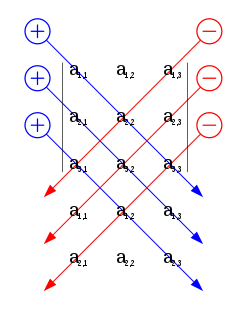
\includegraphics[scale=0.5]{Regla_de_Sarrus.png}
    \caption{Regla de Sarrus}
    \label{sarrus}
\end{figure}


Esta regla intenta emular el caso de orden dos, donde cada sumando es el producto de las diagonales, donde el signo del sumando depende de la direcci\'on de la fecha.

\begin{ejem}
Calcule el determinante de $A = \begin{pmatrix} 5 & -3 & 2 \\ 1 & 0 & 2 \\ 2 & -1 & 3 \end{pmatrix}$
\end{ejem}


\begin{ejem}
Calcule el determinante de $A = \begin{pmatrix} 2 & -3 & 5 \\ 1 & 0 & 4 \\ 3 & -3 & 9 \end{pmatrix}$
\end{ejem}

La siguiente definici\'on nos permitir\'a calcular determinantes de orden superior.
\begin{defin}
Sea $A$ una matriz de $n \times n$. La matriz $M_{ij}$ de $(n-1) \times (n-1)$ que se obtiene de $A$ eliminando la fila $i$ y la columna $j$ se llama el menor $ij$ de $A$.

Sea $A$ una matriz de $n \times n$. El cofactor $ij$ de $A$, denotado por $A_{ij}$ está dado por $A_{ij} = (-1)^{i+j}|M_{ij}|$.
\end{defin}

\begin{ejer}
\begin{enumerate}
    \item Sea $A = \begin{pmatrix} 2 & -1 & 4 \\ 0 & 1 & 5 \\ 6 & 3 & -4 \end{pmatrix}$, calcule $M_{13}$ y $M_{32}$.
    \item Sea $A = \begin{pmatrix} 1 & -3 & 5 & 6 \\ 2 & 4 & 0 & 3 \\ 1 & 5 & 9 & -2 \\ 4 & 0 & 2 & 7 \end{pmatrix}$. Calcule $A_{32}$.
\end{enumerate}
\end{ejer}


\begin{defin}
Sea $A$ una \textbf{matriz de orden $n$}. Entonces el \textbf{determinante de $A$}, denotado por $\det A$ o $|A|$
\begin{align*}
    \det: \M_{n}(K)&\to K\\
    A & \mapsto \det(A)
\end{align*}
y está dado por 
\[\det A = a_{11}A_{11}+a_{12}A_{12}+a_{13}A_{13} + \dots + a_{1n}A_{1n}.\]
\end{defin}

\begin{ejer}
Calcule el determinante de $A$
$$A = \begin{pmatrix} 2 & -3 & 0 & 1 \\ 5 & 4 & 2 & 0 \\ 1 & -1 & 0 & 3 \\ -2 & 1 & 0 & 0 \end{pmatrix}.$$
\end{ejer}





\begin{rec}
Una matriz cuadrada se denomina triangular superior si todas sus componentes abajo de la diagonal son cero. Es una matriz triangular inferior si todas sus componentes arriba de la diagonal son cero. Una matriz se denomina diagonal si todos los elementos que no se encuentran sobre la diagonal son cero.
\end{rec}

\begin{ejem}

$A = \begin{pmatrix} 2 & 1 & 7 \\ 0 & 2 & -5 \\ 0 & 0 & 1 \end{pmatrix}$; $B = \begin{pmatrix} 5 & 0 & 0 \\ 2 & 3 & 0 \\ -1 & 2 & 4 \end{pmatrix}$; $C = \begin{pmatrix} 2 & 0 & 0 \\ 0 & -7 & 0 \\ 0 & 0 & -4 \end{pmatrix}$
\end{ejem}






\begin{thm}
\begin{enumerate}
    \item Sea $A$ una matriz de $n \times n$ triangular superior o inferior. Entonces $\det A = a_{11}a_{22}a_{33} \cdots a_{nn}$.
    \item Sea $T$ una matriz triangular superior. Entonces $T$ es invertible si y solo si $\det T \not= 0$.
    \item Sean $A$ y $B$ dos matrices de orden $n$. Entonces $\det AB = (\det A) (\det B)$.
    \item $\det A^{t} = \det A$.
    \item Si cualquier fila o columna de $A$ es un vector cero, entonces $\det A = 0$.
    \item Si la fila $i$ o columna $j$ de $A$ se multiplica por un escalar $c$, entonces $\det A$ se multiplica por $c$.
\end{enumerate}
\end{thm}

\begin{ejem}
\begin{enumerate}
    \item $\begin{vmatrix} 2 & 1 & 7 \\ 0 & 2 & -5 \\ 0 & 0 & 1 \end{vmatrix} = (2)(2)(1) = 4$.
    \item Sean $A = \begin{pmatrix} 1 & -1 & 2 \\ 3 & 1 & 4 \\ 0 & -2 & 5 \end{pmatrix}$ y $B = \begin{pmatrix} 1 & -2 & 3 \\ 0 & -1 & 4 \\ 2 & 0 & -2 \end{pmatrix}$. Entonces, $\det A = 16$, $\det B = -8$ y $AB = \begin{pmatrix} 5 & -1 & -5 \\ 11 & -7 & 5 \\ 10 & 2 & -18 \end{pmatrix}$

Luego $\det AB = -128 = 16(-8) = (\det A) (\det B)$.

    \item $\begin{vmatrix} -1 & 3 & 0 & 1 \\ 4 & 2 & 0 & 5 \\ -1 & 6 & 0 & 4 \\ 2 & 1 & 0 & 1 \end{vmatrix} = 0$.
    \item Sean $A = \begin{pmatrix} 1 & -1 & 2 \\ 3 & 1 & 4 \\ 0 & -2 & 5 \end{pmatrix}$ y $C = \begin{pmatrix} 1 & -1 & 2 \\ -6 & -2 & -8 \\ 0 & -2 & 5 \end{pmatrix}$. 

Entonces $\det A = 16$ y $\det C = -32 = -2 \det A$
\end{enumerate}
\end{ejem}

\begin{rmk}
El intercambio de dos filas o columnas distintas de $A$ tiene el efecto de multiplicar $\det A$ por $-1$.
\end{rmk}
\begin{ejem}
Sean $A = \begin{pmatrix} 1 & -1 & 2 \\ 3 & 1 & 4 \\ 0 & -2 & 5 \end{pmatrix}$ y $C = \begin{pmatrix} 1 & -1 & 2 \\ 0 & -2 & 5 \\ 3 & 1 & 4 \end{pmatrix}$. 

Luego $\det A = 16$ y $\det C = -16 = - \det A$.
\end{ejem}

\begin{ejer}
\begin{enumerate}
\item Calcule el determinante de la matriz identidad de orden $n$. 
    \item Si $A$ es una matriz de orden $n$ y $k$ es un n\'umero natural. Determine $\det(A^k)$ y $\det(kA)$.
    \item Calcule el determinate de la matriz
    \[A=\begin{pmatrix} 1 & 1 & 1 \\ a & b & c \\ a^2 & b^2 & c^2 \end{pmatrix}\]
    \vspace*{0.5cm}
\end{enumerate}
\end{ejer}



\begin{rmk}
Si $A$ tiene dos filas o columnas iguales, entonces $\det A=0$.
\end{rmk}

%\begin{ejem}
%\begin{center}
%    $\begin{vmatrix} 1 & -1 & 2 \\ 5 & 7 & 3 \\ 1 & -1 & 2 \end{vmatrix} = 0$
%\end{center}
%\end{ejem}

\begin{rmk}
Si una fila o columna de $A$ es un múltiplo escalar de otra fila o columna, entonces $\det A = 0$.
\end{rmk}

\begin{ejem}
    $\begin{vmatrix} 2 & 4 & 1 & 12 \\ -1 & 1 & 0 & 3 \\ 0 & -1 & 9 & -3 \\ 7 & 3 & 6 & 9 \end{vmatrix} = 0$
\end{ejem}




\begin{ejem}
    Calcule $\begin{vmatrix} 1 & 3 & 5 & 2 \\ 0 & -1 & 3 & 4 \\ 2 & 1 & 9 & 6 \\ 3 & 2 & 4 & 8 \end{vmatrix}$
\end{ejem}

\subsection{Matriz adjunta y c\'alculo de la inversa de una matriz}
Ahora podemos generalizar lo visto para matrices de orden 2.
\begin{thm}
Si $\det A = 0$, entonces la matriz $A$ no es invertible. En caso contrario $\det A^{-1} = \frac{1}{\det A}$.
\end{thm}


\begin{defin}
Sea $A$ una matriz de $n \times n$ y sea 
$B =  \begin{pmatrix} A_{11} & A_{12} & \cdots & A_{1n} \\ A_{21} & A_{22} & \cdots & A_{2n} \\ \vdots & \vdots & & \vdots \\  A_{n1} & A_{n2} & \cdots & A_{nn} \end{pmatrix}$, la matriz de sus cofactores. 

Entonces, la adjunta de $A$, escrito $\adj A$, es la transpuesta de la matriz $B$ de $n \times n$, es decir 

\[\adj A = B^t = \begin{pmatrix} A_{11} & A_{21} & \cdots & A_{n1} \\ A_{12} & A_{22} & \cdots & A_{n2} \\ \vdots & \vdots & & \vdots \\  A_{1n} & A_{2n} & \cdots & A_{nn} \end{pmatrix}.\]
\end{defin}





\begin{ejem}
Sea $A =  \begin{pmatrix} 2 & 4 & 3 \\ 0 & 1 & -1 \\ 3 & 5 & 7 \end{pmatrix}$. Calcule $\adj(A)$
\end{ejem}




\begin{thm}
Sea $A$ una matriz de $n \times n$. Entonces $A(\adj A) = (\det A)I_n$.
\end{thm}

\begin{thm}
Sea $A$ una matriz de $n \times n$. Entonces $A$ es invertible si y solo si $\det A \not= 0$. Si $\det A \not= 0$, entonces $A^{-1} = \frac{1}{\det A}\adj A$.
\end{thm}





\begin{ejem}
Sea $A =  \begin{pmatrix} 2 & 4 & 3 \\ 0 & 1 & -1 \\ 3 & 5 & 7 \end{pmatrix}$. Calcule $A^{-1}$.
\end{ejem}



\begin{thm}
\textbf{(Resumen)} Sea $A$ una matriz de $n \times n$. Las siguientes afirmaciones son equivalentes:

\begin{enumerate}
\item
$A$ es invertible


\item
$A$ es equivalente por filas a la matriz identidad de $n \times n$.

\item
La forma escalonada por filas de $A$ tiene $n$ pivotes.

\item
$\det A \not = 0$.
\end{enumerate}
\end{thm}


\begin{subsection}{Optimizaci\'on del c\'alculo de determinante}
Una de las aplicaciones del escalonamiento es el cálculo del valor de un determinante recurriendo a las operaciones elementales.  Será preciso formalizar algunas propiedades que nos aseguren obtener el valor del determinante original mediante matrices equivalentes en las cuales el cálculo resulte sencillo o inmediato. Además, veremos que combinando apropiadamente estas propiedades con el desarrollo por cofactores se logrará gran eficacia y simplicidad en los cálculos.

\begin{thm}
Si se suma un múltiplo escalar de una fila o columna de $A$ a otra fila o columna de $A$, entonces el determinante no cambia. Es decir, el determinante el invariante por operaciones fila suma
\[|A|=|A_{F_i+\alpha F_j}|.\]
\end{thm}
Recordemos que esto \textbf{no es cierto} para la operaci\'on mulplicar por un $\alpha$, m\'as a\'un
\[|A|=\alpha^{-1}|A_{\alpha F_i}|.\]

\begin{ejer}
Obtenga el valor de $ \begin{vmatrix} x & y & z \\ 3x+3 & 3y & 3z+2 \\ x+4 & y+4 & z+4 \end{vmatrix}$ sabiendo que $ \begin{vmatrix} x & y & z \\ 3 & 0 & 2 \\ 1 & 1 & 1 \end{vmatrix}=1$.
    \vspace*{0.5cm}
\end{ejer}
Si recordamos que $|A^t| = |A|$, se nos hará evidente que, en el cálculo de un determinante, las propiedades mencionadas para las operaciones elementales entre filas serán homólogas para las operaciones elementales entre columnas. Incluso se pueden aplicar en forma combinada unas y otras.

Por lo tanto, si usamos estas tres operaciones, ya sea entre filas o entre columnas, para construir la escalonada asociada a A  que no es otra que la triangular superior equivalente , obtendremos el valor para $|A|$ multiplicando los elementos de la diagonal principal de esa triangular.


\begin{ejer}
Sea $A_\alpha=\begin{vmatrix} 2 & 1 & 4 \\ 1 & \alpha-1 & 2\\ 2 & 1 & \alpha+1  \end{vmatrix}$. Encuentre los valores de $\alpha$, de manera que la matriz $A_\alpha$ sea invertible.
\end{ejer}
Otra propiedad interesante del determinante es la siguiente
\begin{thm}
Si todos los elementos de una fila de una matriz se descomponen en la suma de dos sumandos, el
determinante de la matriz inicial es la suma de dos determinantes que tienen en una fila, respectivamente, el
primer y segundo sumando, siendo el resto de las filas iguales a las filas del determinante de la matriz inicial. Es decir,
\[\begin{vmatrix} \alpha+ a & \beta + b & \gamma + c \\ a_{12} & a_{22}  & a_{32}  \\  a_{13} & a_{23}  & a_{33} \end{vmatrix}=\begin{vmatrix} \alpha& \beta  & \gamma  \\ a_{12} & a_{22}  & a_{32}  \\  a_{13} & a_{23}  & a_{33} \end{vmatrix}+\begin{vmatrix}  a &  b &  c \\ a_{12} & a_{22}  & a_{32}  \\  a_{13} & a_{23}  & a_{33} \end{vmatrix}.\]
\end{thm}
\end{subsection}




\section{Sistema de Ecuaciones Lineales.}
Objetivos:
\begin{itemize}
    \item Estudiar sistemas de ecuaciones lineales.
    \item Aprender a utilizar el método de la reducción gaussiana para resolver sistemas de ecuaciones algebraicas.
    \item Aprender a utilizar el método de la reducción de Gauss-Jordan para resolver sistemas de ecuaciones algebraicas.
    \item Aprender los sistemas homogéneos y las características de su solución.
    \item Relacionar matrices y vectores con sistemas de ecuaciones.
    \item Determinar condiciones para la existencia de soluciones de sistemas de ecuaciones homogéneos y no homogéneos.
\end{itemize}
\subsection{Introducción a los sistemas lineales.}

\begin{defin}
Se define una ecuación lineal de $n$ variables sobre un cuerpo $(K, +, ·)$
como una igualdad de la forma: 
\[a_1\cdot x_1 + a_2\cdot x_2 + \dots  + a_n\cdot x_n = b,\]
donde cada $x_j$ es variable incógnita de la ecuación, cada $a_j$ es coeficiente numérico (en $K$)
para la $j-$ésima variable $(x_j)$ y $b$ es la constante (en $K$) que resulta de la suma ponderada (por $a_j$) de las variables $x_j$. De manera abreviada
\[\sum_{j=1}^n a_j \cdot x_j=b\]
\end{defin}
Su resolución consiste en determinar todas y cada una de las $n-$uplas $(s_1, s_2,\dots, s_n )$ de valores
$s_j$ asignados a cada variable $x_j$ para satisfacer la igualdad, es decir 
\[\sum_{j=1}^n a_j \cdot s_j=b\]
Luego, el conjunto solución se anotaría:

\[S_E=\left\{(s_1, s_2,\dots, s_n )\in K^n \colon \sum_{j=1}^n a_j \cdot s_j=b\right\}\]

\begin{ejem}
$3x_1 - 2x_2 + 7x3 - x_4 = 9$ es una ecuación lineal de 4 variables.
$(-1, 2, 3, 5 )$ es \textbf{una} solución o un elemento del conjunto solución puesto que : $3(-1) - 2(2) + 7(3) -(5)$ resulta igual a 9.

Verifique usted que $(2, 3, -2, -23)$ es otra solución para nuestra ecuación.
Note que hay una infinidad de cuádruplas en la solución $S_E$ de nuestra ecuación.
\end{ejem}

Es muy frecuente que nos interese resolver problemas que exigen satisfacer varias
condiciones (ecuaciones) simultáneas por parte de un cierto número $n$ de variables
(incógnitas). En este caso, se habla de resolver una familia de $m$ ecuaciones para esas
incógnitas. Como la resolución debe ser simultánea, el conjunto solución (de $n-$uplas) para
el sistema de ecuaciones resultará coincidente con la intersección de los $m$ conjuntos
solución para cada una de esas $m$ ecuaciones.

\begin{defin}
Un \textbf{sistema de $m$ ecuaciones con $n$ incógnitas} es un sistema que se escribe de la siguiente forma:
\[\begin{array}{ccccccc}
        a_{11}x_1&+ a_{12} x_2&+ \dots &+ a_{1j}x_j &+ \dots &+ a_{1n}x_n=& b_1\\
     a_{21}x_1&+ a_{22} x_2&+ \dots &+ a_{2j} x_j&+\dots &+  a_{2n}x_n=& b_2\\
    \vdots & \vdots &  & \vdots  &  &\dots  & \vdots\\
     a_{m1}x_1&+ a_{m2} x_2&+ \dots&+  a_{mj}x_j&+ \dots&+  a_{mn}x_n=& b_m
\end{array}\]
\end{defin}
\begin{rmk}
Note que, respecto de los coeficientes numéricos $a_{ij}$, $i$ nos indica que es coeficiente de la $i-$ésima ecuación y que $j$ nos indica que este coeficiente pondera a la $j-$ésima incógnita.
\end{rmk}
%\begin{ejem}

%Un \textbf{sistema de dos ecuaciones} y dos incógnitas $x$ e $y$ es un sistema de la forma:
%\begin{align}\label{sistema}
% a_{11}x + a_{12}y &= b_1,\\
%a_{21}x + a_{22}y &= b_2,   \nonumber
%\end{align}
%donde $ a_{11}, a_{12},a_{21},a_{22}, b_1$ y $
%b_2$ son n\'umeros dados. 

%Una \textbf{solución al sistema} \ref{sistema} es un par de números, denotados por $(x,y)$, que satisface las igualdades en \ref{sistema}. 

%\end{ejem}

Si interpretamos cada una de las ecuaciones del sistema como una l\'inea recta, la soluci\'on de dicho sistema puede pensarse como la intersecci\'on de las dos rectas en un espacio $n-$dimensional.

Un sistema de ecuaciones lineales tiene ya sea:
\begin{enumerate}
    \item Una solución (el sistema es consistente).
    \item Infinitas soluciones (el sistema es consistente).
    \item Ninguna solución (el sistema es inconsistente).
\end{enumerate}
\begin{ejem}
\begin{enumerate}
    \item Resolver el sistema 
\begin{align*}
    3x -2y &= 4,\\
    5x + 2y &= 12.
\end{align*}
Sumando ambas ecuaciones tenemos que $8x=16$, luego $x=2$. Reemplazando en la primera ecuaci\'on $3\cdot 2-2y=4$, por lo tanto $2=2y$, obteniendo $y=1$. Finalmente la solución única de este sistema de ecuaciones es el vector $(2, 1)$.

Geom\'etricamente las ecuaciones representan dos rectas que se
intersectan en un punto $(2, 1)$.
    
    \item Resolver el sistema 
    \begin{align*}
    x -y &= 7,\\
    2x -2y &= 14.
\end{align*}
Notemos que la segunda ecuaci\'on puede obtenerse multiplicando la primera por dos, por lo tanto las ecuaciones representan la misma recta. Cada punto de la recta es una solución de este sistema. Por lo tanto, este sistema de ecuaciones tiene infinitas soluciones. Como $x -y = 7$, entonces $x = y -7$, luego las soluciones $(x,y)$ son de la forma $(y-7,y)$, obteniendo una soluci\'on por cada $y\in \R$. Por ejemplo, para $y=0$ tenemos el punto $(-7,0)$.

    \item Resolver el sistema 
    \begin{align*}
    x -y &= 7,\\
    2x -2y &= 13.
\end{align*}
Si asumimos que existe una soluci\'on, al restar ambas ecuaciones obtenemos $0=1$, lo que claramente es una contradicci\'on, por lo tanto, este sistema de ecuaciones no puede tener solución. En este caso, las ecuaciones representan dos rectas paralelas que no se intersectan.
\end{enumerate}
\end{ejem}

\begin{defin}
Si contamos con dos sistemas de ecuaciones que al menos coinciden en que sus incógnitas son las mismas, es decir, 
\[\sum_{j=1}^n a_j \cdot x_j=b_i,\]
con $1 \leq  i \leq  m$ y
\[\sum_{j=1}^n \alpha_j \cdot x_j=\beta_i\]
con $1 \leq  i \leq  p$ ; diremos que ellos son \textbf{equivalentes} cuando
y sólo cuando su conjunto solución sea el mismo.
\end{defin}





\subsection{Métodos directos para resolver sistemas lineales.}

En en caso particular de un sistema de $3\times 3$ podemos resolver dicho sistema siguiendo la siguiente estrategia:
\begin{enumerate}
    \item Dividir la primera ecuación, entre una constante, para hacer el coeficiente de $x_1$ igual a 1.
    \item Multiplicar la primera ecuación por las constantes adecuadas de modo que al sumarla a la segunda y tercera ecuaciones, respectivamente, se eliminen los términos en $x_1$.
    \item Dividir la segunda ecuación entre una constante, para hacer el coeficiente de $x_2$ igual a 1 y después usarla para eliminar los términos en $x_2$ de la primera y tercera ecuaciones.
    \item Dividir la tercera ecuación entre una constante, para hacer elcoeficiente de $x_3$ igual a 1 y después usarla para eliminar los términos de $x_3$ de la primera y segunda ecuaciones.
\end{enumerate}



\subsection{Sistemas de $m$ Ecuaciones con $n$ Incógnitas}
Al sistema 
\[\begin{array}{ccccccc}\label{nsistema}
        a_{11}x_1&+ a_{12} x_2&+ \dots &+ a_{1j}x_j &+ \dots &+ a_{1n}x_n=& b_1\\
     a_{21}x_1&+ a_{22} x_2&+ \dots &+ a_{2j} x_j&+\dots &+  a_{2n}x_n=& b_2\\
    \vdots & \vdots &  & \vdots  &  &\dots  & \vdots\\
     a_{m1}x_1&+ a_{m2} x_2&+ \dots&+  a_{mj}x_j&+ \dots&+  a_{mn}x_n=& b_m
\end{array}\]
$m$ ecuaciones con $n$ incógnitas se puede representar matricialmente de la forma:
\[\left(\begin{array}{cccc}
     a_{11}& a_{12} & \dots  & a_{1n}\\
     a_{21}& a_{22} & \dots & a_{2n}\\
     \vdots&  \vdots &    &  \vdots\\
     a_{m1}& a_{m2}  &\dots & a_{mn}
\end{array}\right) \left(\begin{array}{c}
   x_1 \\
   x_2 \\
   \vdots\\
   x_n 
\end{array}\right)= \left(\begin{array}{c}
   b_1 \\
   b_2 \\
   \vdots\\
   b_n 
\end{array}\right)\]
Es decir, si $A=(a_{ij})$, $x=(x_j)$ y $b=(b_j)$, entonces el sistema anterior es equivalente a $Ax=b$.

\begin{defin}
A la matriz $(A|b)$ se le conoce como la matriz aumentada del sistema de ecuaciones.
\end{defin}
Esta matriz ser\'a \'util en el estudio del n\'umero de soluciones que tiene el sistema y eventualmente determinar el conjunto soluci\'on.

\subsection{Métodos para resolver sistemas de ecuaciones:}

A partir de la matriz aumentada $(A| b)$ se puede resolver al sistema de ecuaciones lineales $Ax = b$, con $A\in \M_{m\times n}$ por lo menos de dos formas que usan del escalonamiento por filas. También se le podrá resolver usando determinantes cuando el sistema tenga igual número de ecuaciones e incógnitas.

La elección de uno u otro método dependerá de las características de tamaño del
sistema a resolver, de sus coeficientes numéricos, de los recursos con que se cuente y,
obviamente, de lo que se pretenda obtener del sistema. Es la práctica la que nos dará
criterios para hacer una buena elección de método.



\begin{itemize}
\item
Eliminación Gaussiana

\begin{enumerate}
\item
Utilizar operaciones filas para reducir la matriz aumentada del sistema a su forma escalonada por filas, hasta obtener la matriz escalonada por filas $(E| g)$ que se asocia al sistema $Ex=g$, que resulta ser equivalente al sistema inicial, es decir ambos sistemas tienen las mismas soluciones.

\item
Despejar el valor de la última incógnita y después utilizar la sustitución hacia atrás para las demás incógnitas.
\end{enumerate}

\item
Eliminación de Gauss Jordan

\begin{enumerate}
\item
Utilizar operaciones filas para reducir la matriz aumentada del sistema a su forma escalonada reducida por filas $(R| s)$.

\item
Si el sistema es consistente, resolver para las variables principales en términos de las variables libres restantes.
\end{enumerate}
\end{itemize}

\begin{rmk}
\begin{enumerate}
    \item Si en el sistema $A·x = b$, con $A\in\M_{m\times n}$, ocurre que su equivalente $(E| g)$ es de rango
$r$ ($r$ filas no nulas), \textbf{habrá $r$ incógnitas dependientes en el sistema y, por ende, $n - r$ incógnitas independientes de las que dependerá el conjunto solución}.
Si resulta que el rango de $(E| g) = n$, que corresponde al n\'umero de variables, entonces todas las incógnitas son
dependientes o determinadas y la solución del sistema $Ax = b$ es única para cada
variable: $x_1= s_1, x_2= s_2, \dots , x_n = s_n$.
\item Si al escalonar $(A| b)$, alguna fila de $(E| g)$ o de $(R| s)$ resulta de la
forma $(0\; 0\; \dots\; 0| g_i \neq 0)$, o $(0\; 0 \;\dots\; 0| s_i \neq 0)$, significa que alguna ecuación del sistema original era contradictoria con las demás puesto que habría una ecuación del tipo $0·x_1 + 0·x_2 + \dots 0·x_n \neq 0$ lo que es imposible. En estos casos, diremos que la solución no existe y que el sistema es
inconsistente o que las ecuaciones son incompatibles. Dicho de otro modo,
la solución será vacía cuando el rango de $A$ sea menor que el rango de $(A|
b)$.
\item Cuando el rango $A$ es igual con el rango de $(A| b)$, podemos concluir que este rango nos indica el número de ecuaciones independientes existentes entre $m$ ecuaciones originales. Todas las filas nulas en $(E| g)$ o $(R| s)$ nos dicen que las ecuaciones asociadas a esas filas eran ecuaciones dependientes o Redundantes, ya que imponían a las variables una condición que ya era exigida por las otras ecuaciones.
\end{enumerate}
Todo lo anterior se puede resumir en el siguiente teorema.
\begin{thm}[Rouché–Frobenius]
Existen soluciones para el sistema si y solo si el rango de la matriz aumentada es igual al rango de la matriz $A$.
Luego,
\[rank(A) < rank(A|b)\Longrightarrow S_S = \emptyset\]
Entonces, si existen soluciones, es decir $rank(A) = rank(A|b)$, tenemos dos situaciones:
\begin{enumerate}
    \item Si el rango de $A$ es $n$, entonces la solución es única. M\'as a\'un, se tiene que $A$ es invertible y $x = A^{-1}b$.
    \item Si $rank(A) = rank(A|b)<n$ existen infinitas soluciones.
\end{enumerate}
\end{thm}


\end{rmk}


\begin{ejer}
Resuelva

\begin{enumerate}
\item
\begin{equation*}
\systeme{
w - x - y + 2z = 1,
2w - 2x - y + 3z = 3,
-w + x - y = -3
}
\end{equation*}


\item
\begin{equation*}
\systeme{
 x_1 - 3x_2 - 5x_3 + x_4 = 4,
 2x_1 + 5x_2 - 2x_3 + 4x_4 = 6
}
\end{equation*}
\end{enumerate}
\end{ejer}
Note que el número de
variables libres será la diferencia entre el total de variables y el rango
de $A$.

\begin{ejer}
Estudiemos los valores del parámetro $\alpha\in \R$ para que la familia de sistemas de ecuaciones lineales:
\begin{equation*}
\systeme{
\alpha x + 3y = -\alpha,
2\alpha x + 5y -\alpha^2 z= 0,
2\alpha x + 5y-z = \alpha +1
}
\end{equation*}
de manera que tenga tenga una solución : i) única ; ii) vacía ; ó, iii) infinitas soluciones.
\end{ejer}




\subsection{Regla de Cramer}

Un sistema de $n$ ecuaciones con $n$ incógnitas: 

$$\begin{matrix} a_{11}x_1 & + & a_{12}x_2 & + & \cdots & + & a_{1n}x_n & = & b_1 \\ a_{21}x_1 & + & a_{22}x_2 & + & \cdots & + & a_{2n}x_n & = & b_2 \\ \vdots & & \vdots & & & & \vdots & & \vdots \\ a_{n1}x_1 & + & a_{n2}x_2 & + & \cdots & + & a_{1n}x_n & = & b_n \end{matrix}$$

se puede escribir de la forma $Ax = b$.


Si $\det A \not= 0$, el sistema tiene solución única. 

Sea $D = \det A$, definamos:


$A_1 = \begin{pmatrix} b_1 & a_{12} & \cdots & a_{1n} \\ b_2 & a_{22} & \cdots & a_{2n} \\ \vdots & \vdots & & \vdots \\ b_n & a_{n2} & \cdots & a_{nn} \end{pmatrix}, A_2 = \begin{pmatrix} a_{11} & b_1 & \cdots & a_{1n} \\ a_{12} & b_2 & \cdots & a_{2n} \\ \vdots & \vdots & & \vdots \\ a_{n1} & b_n & \cdots & a_{nn} \end{pmatrix}, \dots, A_n = \begin{pmatrix} a_{11} & a_{12} & \cdots & b_1 \\ a_{21} & a_{22} & \cdots & b_2 \\ \vdots & \vdots & & \vdots \\ a_{n1} & a_{n2} & \cdots & b_n \end{pmatrix}$.
\\\

y sean $D_1 = \det A_1$, $D_2 = \det A_2$,$\dots, D_n = \det A_n$.


\begin{thm}
Sea $A$ una matriz de $n \times n$ y suponga que $\det A \not= 0$. Entonces la solución única al sistema $Ax = b$ está dada por:

$$x_1 = \frac{D_1}{D}, x_2 = \frac{D_2}{D}, \cdots, x_i = \frac{D_i}{D}, \cdots, x_n = \frac{D_n}{D}$$
\end{thm}


\begin{ejer}
Resuelva el siguiente sistema de ecuaciones utilizando la Regla de Cramer:

\begin{equation*}
\systeme{
2x_1+4x_2+6x_3=18,
4x_1+5x_2+6x_3=24,
3x_1+x_2-2x_3=4
}
\end{equation*}

\end{ejer}

\subsection{Sistemas Lineales Homogéneos}
\begin{defin}
Un sistema de $m \times n$ ecuaciones lineales se llama homogéneo si todas las constantes $b_1,b_2, \dots , b_m$ son cero. Si una o más de las constantes es diferente de cero, decimos que el sistema lineal es no homogéneo.

$$\begin{matrix} a_{11}x_1 &+ & a_{12}x_2 & + & \cdots & + & a_{1n}x_n & = & 0 \\ a_{21}x_1 & + & a_{22}x_2 & + & \cdots & + & a_{2n}x_n & = & 0 \\ \vdots & & \vdots & & &  & \vdots & & \vdots \\ a_{m1}x_1 & + & a_{m2}x_2 & + & \cdots & + & a_{mn}x_n & = & 0 \end{matrix}$$
\end{defin}

\begin{ejem}
\begin{enumerate}
\item
\begin{equation*}
\systeme{
2x_1 + 4x_2 + 6x_3 = 0,
4x_1 + 5x_2 + 6x_3 = 0,
3x_1 + x_2 - 2x_3 = 0
}
\end{equation*}

\item
\begin{equation*}
\systeme{
x_1 + 2x_2 - x_3 = 0,
3x_1 - 3x_2 + 2x_3 = 0,
-x_1 - 11x_2 + 6x_3 = 0
}
\end{equation*}
\end{enumerate}
\end{ejem}


\begin{thm}
Un sistema homogéneo tiene un número infinito de soluciones si tiene más incógnitas que ecuaciones, es decir, si $m < n$.
\end{thm}

\begin{thm}
Sean $x_1$ y $x_2$ dos soluciones al sistema no homogéneo $Ax=b$. Entonces su diferencia $x_1-x_2$ es una solución al sistema homogéneo asociado $Ax= \textbf{0}$.
\end{thm}

\begin{cor}
Sea $x$ una solución particular al sistema no homogéneo y sea $y$ otra solución. Entonces existe una solución $h$ al sistema homogéneo tal que: $y = x + h$.
\end{cor}


\begin{thm}
\textbf{(Resumen)} Sea $A$ una matriz de $n \times n$. Las siguientes afirmaciones son equivalentes:

\begin{enumerate}
\item
$A$ es invertible

\item
La única solución al sistema homogéneo $Ax = 0$ es la solución trivial.

\item
El sistema $Ax = b$ tiene una solución única para cada vector de dimensión $n$ $b$.

\item
$A$ es equivalente por filas a la matriz identidad de $n \times n$.

\item
La forma escalonada por filas de $A$ tiene $n$ pivotes.

\item
$\det A \not = 0$.
\end{enumerate}
\end{thm}

\begin{thm}
Una condición necesaria y suficiente para que $Ax = 0$, sistema de
ecuaciones lineales homogéneas con $n$ variables incógnitas, tenga al menos
una solución diferente de cero es que $rank(A) < n$.
\end{thm}

\textbf{Consecuencias:}
\begin{enumerate}
    \item Si el sistema homogéneo $Ax = 0$, es tal que $rank (A) = n$, o que $|A| \neq 0$, o que $A$ es
invertible, entonces tiene solución trivial es decir $S_H = \{x=(0, \dots, 0) \}$.
\item Si $Ax = 0$ es tal que tiene menos ecuaciones que incógnitas entonces tiene
solucion no trivial, es decir $S_H$ tiene infinitas soluciones.
\item Si $Ax = 0$ es tal que tiene igual número de ecuaciones que de incógnitas entonces:
\begin{enumerate}
    \item Si $|A| \neq 0$ , entonces $S_H = \{0 \}$
    \item  Si $|A| = 0 $, entonces $S_H$ tiene infinitas soluciones.
\end{enumerate}
\item Si $Ax = 0$ tiene al menos una solución no trivial entonces:
\begin{enumerate}
    \item Si $x_0\in S_H$, es decir, es solución del sistema homogéneo, entonces $\lambda x_0 \in S_H$ para todo $\lambda \in K$, pues $A(\lambda x_0) = \lambda(A x_0) = \lambda 0 = 0$.
    \item  Si $x_1 , x_2 \in S_H$ entonces $x_1 + x_2 \in S_H $, pues $Ax_1 = 0$ y $Ax_2 = 0$ entonces
$A(x_1 + x_2 ) = Ax_1 + Ax_2 = 0 + 0 = 0$.
\end{enumerate}
De lo anterior, se concluye que si $Ax = 0$ tiene una solución no trivial entonces
tiene infinitas soluciones.
\end{enumerate}

\section{Diagonalizaci\'on}
Una matriz cuadrada \( A \in \mathbb{R}^{n \times n} \) se dice que es \textbf{diagonalizable} si existe una matriz invertible \( P \in \mathbb{R}^{n \times n} \) y una matriz diagonal \( D \in \mathbb{R}^{n \times n} \) tal que:
\[
A = P D P^{-1}
\]

En los próximos capítulos veremos las condiciones necesarias y suficientes de manera que la matriz sea diagonalizable. Por el momento, sólo describiremos el procedimiento para encontrar las matrices $P$ y $D$.
% Una matriz \( A \) es diagonalizable si y sólo si tiene un conjunto completo de \( n \) vectores propios linealmente independientes, es decir, si existe una base del espacio \( \mathbb{R}^n \) formada por vectores propios de \( A \).
\begin{defin}
    Sea \( A \in \mathbb{R}^{n \times n} \) una matriz cuadrada. Un número \( \lambda \in \mathbb{R} \) se llama \textbf{valor propio} (o \textit{autovalor}) de la matriz \( A \) si existe un vector no nulo \( \vec{v} \in \mathbb{R}^n \), llamado \textbf{vector propio} (o \textit{autovector}), tal que:

\[
A\vec{v} = \lambda \vec{v}
\]

Esta ecuación puede reescribirse como un sistema homogéneo:

\[
(A - \lambda I)\vec{v} = \vec{0}
\]

donde \( I \) es la matriz identidad de orden \( n \). 

Entonces, \( \lambda \) es un valor propio de \( A \) si y sólo si el sistema homogéneo:

\[
(A - \lambda I)\vec{v} = \vec{0}
\]

tiene soluciones no triviales (es decir, \( \vec{v} \neq \vec{0} \)).

Esto ocurre si y sólo si la matriz \( (A - \lambda I) \) es \textbf{invertible}, es decir:

\[
\det(A - \lambda I) = 0
\]

Una vez encontrado un valor propio \( \lambda \), los vectores propios asociados se obtienen resolviendo el sistema lineal homogéneo:

\[
(A - \lambda I)\vec{v} = \vec{0}
\]

\textbf{Nota:} El conjunto de soluciones no triviales de este sistema forma un subespacio vectorial llamado \textit{espacio propio} asociado al valor propio \( \lambda \), pero esto se desarrollará en los capítulos siguientes.
\end{defin}



\subsection*{Procedimiento para Diagonalizar una Matriz}
Dado \( A \in \mathbb{R}^{n \times n} \):

\begin{enumerate}
    \item Calcular los valores propios (\( \lambda \)) resolviendo el \textbf{polinomio característico} dado por:
    \[
    \det(A - \lambda I) = 0
    \]
    
    \item Para cada valor propio \( \lambda_i \), encontrar los vectores propios resolviendo:
    \[
    (A - \lambda_i I)\vec{v} = 0
    \]
    
    \item Si se obtienen \( n \) vectores propios distintos, entonces:
    \[
    P = [\vec{v}_1 \; \vec{v}_2 \; \cdots \; \vec{v}_n], \quad D = \text{diag}(\lambda_1, \lambda_2, \ldots, \lambda_n)
    \]
    
    \item Finalmente:
    \[
    A = P D P^{-1}
    \]
\end{enumerate}

\begin{ejem}
    Sea 
\[
A = \begin{pmatrix}
4 & 1 \\
0 & 2
\end{pmatrix}
\]

\textbf{Paso 1:} Polinomio característico:
\[
\det(A - \lambda I) = \det \begin{pmatrix}
4 - \lambda & 1 \\
0 & 2 - \lambda
\end{pmatrix} = (4 - \lambda)(2 - \lambda)
\]
Valores propios: \( \lambda_1 = 4, \; \lambda_2 = 2 \)

\textbf{Paso 2:} Vectores propios:

Para \( \lambda = 4 \):
\[
(A - 4I)\vec{v} = 0 \Rightarrow \begin{pmatrix}
0 & 1 \\
0 & -2
\end{pmatrix} \vec{v} = 0 \Rightarrow \vec{v}_1 = \begin{pmatrix}1 \\ 0\end{pmatrix}
\]

Para \( \lambda = 2 \):
\[
(A - 2I)\vec{v} = 0 \Rightarrow \begin{pmatrix}
2 & 1 \\
0 & 0
\end{pmatrix} \vec{v} = 0 \Rightarrow \vec{v}_2 = \begin{pmatrix}-1 \\ 2\end{pmatrix}
\]

\textbf{Paso 3:} Matrices \( P \) y \( D \):

\[
P = \begin{pmatrix}
1 & -1 \\
0 & 2
\end{pmatrix}, \quad D = \begin{pmatrix}
4 & 0 \\
0 & 2
\end{pmatrix}
\]

\textbf{Verificación:} \( A = P D P^{-1} \)
\end{ejem}

\section{Espacios Vectoriales}

\textbf{Objetivos del Capítulo}

\begin{itemize}
\item
Aprender la definici\'on de un espacio vectorial real.

\item
Estudiar el concepto de subespacio vectorial.

\item
Familiarizarse con la operación de combinación lineal y el concepto de espacio generado.

\item
Conocer la propiedad de independencia lineal.

\item
Profundizar en el conjunto mínimo de vectores con los que se puede generar un espacio vectorial. Para definir el concepto de bases y dimensiones de un espacio vectorial.

\item
Expresar vectores con bases diferentes.

\item
Aprender a definir conceptos relacionados con subespacios vectoriales formados a partir de las filas y las columnas de matrices.

\end{itemize}



\subsection{Definición y Propiedades Básicas}

Durante toda esta secci\'on, denotaremos por $K$ un \emph{cuerpo}, esto es de un conjunto con dos leyes de composici\'on, denotadas $+$ y $\cdot$, y dos elementos especiales 0 y 1, distintos entre s\'i, que cumplen las siguientes
propiedades:

\begin{enumerate}
    \item $+$ y $\cdot$ son asociativas;
    \item $+$ y $\cdot$ son conmutativas;
    \item $\cdot$ es distributiva con respecto a $+$;
    \item $0$ es el neutro de $+$ y $1$ es el neutro de $\cdot$;
    \item para todo $a \in K$, existe $a'\in  K$ tal que $a + a'=0$ (usualmente $a'$ se denota por $-a$);
    \item para todo $a \in K\setminus \{0\}$, existe $a \in K \setminus \{0\}$ tal que $a \cdot a' = 1$ (usualmente $a''$ se denota $a^{-1}$ o $1/a$).
\end{enumerate}
Si bien esta definici\'on es general, durante el curso consideraremos $K$ igual a $\Q, \R$ o $\C$.

Sea $(K, +, \cdot)$ un cuerpo. Comencemos con la definici\'on de un espacio vectorial.
\begin{defin}

Un $K-$espacio vectorial (o espacio vectorial sobre $K$) es un
conjunto no vac\'io $V$ provisto de dos operaciones binarias 
\begin{align*}
        + : V \times V &\to V &\cdot : K \times V &\to V\\
 (x, y) &\mapsto x + y&  (\alpha, y)& \mapsto \alpha \cdot y
\end{align*}
llamadas respectivamente suma y multiplicación por escalar y que satisfacen las siguientes propiedades:

\begin{enumerate}

\item
$+$ es asociativa, es decir $(x+ y)+ z = x+ (y+ z)$ para todo $x, y, z \in V$.

\item
$+$ es conmutativa, es decir $x + y = y + x$ para todo $x, y \in V$.

\item
$+$ tiene un elemento neutro $0_V$ , es decir $x + 0_V = x = 0_V + x$ para todo
$x \in V$.

\item
$+$ tiene inversos, es decir, para todo $x \in V$ , existe $x' \in V$ tal que $x + x' =0_V$.

\item
$\alpha \cdot  (\beta \cdot  x) = (\alpha \cdot \beta) \cdot  x$ para todo $\alpha , \beta \in K$ y todo $x \in V$.

\item
$(\alpha + \beta) \cdot x = (\alpha \cdot x) + (\beta \cdot x)$ para todo $\alpha,\beta \in K$ y todo $x \in V$.

\item
$\alpha \cdot (x + y) = (\alpha \cdot x) + (\alpha \cdot y)$ para todo $\alpha \in K$ y todo $x, y \in V$.

\item
$1 \cdot x = x$ para todo $x \in V$.
\end{enumerate}
\end{defin}
Los elementos de un espacio vectorial se llaman vectores.
Denotaremos por $(V,+,\cdot, K)$ al $K-$espacio vectorial $V$.



\begin{ejem}
\begin{enumerate}
\item
$\mathbb{R}^2$ es un espacio vectorial sobre $\R$.

\item
$\mathbb{R}^n$ es un espacio vectorial sobre $\R$.

\item
$V= \{ \textbf{0} \}$ es un espacio vectorial sobre cualquier cuerpo.

\item
$V= \{ 1 \}$ No es un espacio vectorial.

\item
$V= \{ (x,y)\in \R^2: y = mx \}$ es un espacio vectorial sobre $\R$.


\item
$V = M_{m\times n}(\R)$ el conjunto de matrices $m\times n$ con coeficientes en $\R$ es
un $\R-$espacio vectorial para la suma de matrices y la  multiplicaci\'on por escalares.

\item $\C$ es un $\R-$espacio vectorial con la suma de complejos y la multiplicaci\'on por escalar dada por $\alpha(a+bi) = \alpha a+\alpha bi$ para todo $\alpha \in \R$ y $(a+bi)\in \C$.
$\C$ es un $C-$espacio vectorial con la suma de complejos y la  la multiplicaci\'on de complejos.
Estos espacios vectoriales son distintos.
\item Definimos el conjunto de todos los polinomios con coeficientes en $K$ con indeterminada $x$ como
\[K[x]=\left\{p(x)=\sum_{i=0}^m a_i x^i\quad\colon a_i\in K, \quad m \in \N\right\},\]
con las operaciones adici\'on y ponderaci\'on definidas por
\begin{enumerate}
    \item $\sum_{i=0}^s a_i x^i+\sum_{i=0}^t b_i x^i=\sum_{i=0}^m (a_i+b_i) x^i$, donde $m=\max\{s,t\}$.
    \item $\alpha\left(\sum_{i=0}^m a_i x^i\right)=\sum_{i=0}^m (\alpha a_i) x^i$.
\end{enumerate}
Con estas operaciones $(K[x],+, \cdot, K)$ es un espacio vectorial.
\item Definimos el conjunto 
\[K_n[x]=\left\{p(x)\in K[x]\colon \deg(p(x))\leq n\right\}.\]
Este conjunto con las operaciones anteriores, es un espacio vectorial sobre $K$.
\item Sea $A\subset \R$ no vac\'io. El conjunto de funciones 
\[\mathcal{F}(A,\R):=\{f:A\to \R\colon f \text{ funci\'on}\},\]
con la suma y poderaci\'on usuales(punto a punto), es un $\R-$espacio vectorial.
\item Sea $A\subset \R$ no vac\'io. El conjunto de funciones continuas
\[\mathcal{C}(A,\R):=\{f:A\to \R\colon f \text{ funci\'on continua}\},\]
con la suma y poderaci\'on usuales, es un $\R-$espacio vectorial.
\item Sea $A\subset \R$ no vac\'io. El conjunto de funciones continuas
\[\mathcal{D}(A,\R):=\{f:A\to \R\colon f \text{ funci\'on derivable}\},\]
con la suma y poderaci\'on usuales, es un $\R-$espacio vectorial.
\end{enumerate}
\end{ejem}

\begin{ejer}
Verifique que los ejemplos anteriores son efectivamente espacios vectoriales sobre los cuerpos correspondientes.
\end{ejer}



\begin{thm}
Sea $V$ un espacio vectorial. Entonces:

\begin{enumerate}
\item
$\alpha \textbf{0} = \textbf{0}$ para todo escalar $\alpha$.

\item
$\textbf{0} \cdot x = \textbf{0}$ para todo $x \in V$.

\item
Si $\alpha x = \textbf{0}$, entonces $\alpha = 0$ o $x = \textbf{0}$ (o ambos).

\item
$(-1)x = -x$ para todo $x \in V$.
\end{enumerate}
\end{thm}
\begin{ejer}
Demuestre las propiedades anteriores.
\end{ejer}
\subsection{Subespacios vectoriales}
\begin{defin}
Se dice que $H$ es un subespacio vectorial de $V$ si $H$ es un subconjunto no vacío de $V$, y $H$ es un espacio vectorial, junto con las operaciones de suma entre vectores y multiplicación por escalar definidas para $V$.
\end{defin}

\begin{thm}
Un subconjunto no vacío de $H$ de un espacio vectorial $V$ es un subespacio de $V$ si se cumplen las siguientes condiciones:

\begin{enumerate}
\item
Si $x \in H$ y $y \in H$, entonces $x + y \in H$.

\item
Si $x \in H$, entonces $\alpha x \in H$ para todo escalar $\alpha$.
\end{enumerate}
\end{thm}

\begin{rmk}
Todo subespacio de un espacio vectorial $V$ contiene al vector $\textbf{0}$.
\end{rmk}

La definici\'on de subespacio se puede reducir a una sola propiedad, que es la siguiente: para todo $\alpha \in K$ y para todo $x, y \in H$, $\alpha x+y \in H$. En efecto, esta propiedad se deduce inmediatamente de (1) y (2). Por otra parte, partiendo de esta propiedad
obtenemos (1) tomando $\alpha = 1$. Con $x = y$ y $\alpha = -1$ obtenemos que $0\in H $, por
lo que podemos tomar $y = 0$ y obtenemos (2). En particular, vemos que todo
subespacio vectorial contiene a $0$.




\begin{ejem}
\begin{enumerate}
\item
$H = \{ \textbf{0} \}$.

\item
Todo espacio vectorial es subespacio de sí mismo.


\item
Sea $V = \mathbb{R}^2$. Un subespacio vectorial de $V$ es $H = \{ (x,y): y = mx \}$.


\item
Demuestre que $H_1 = \{(x,y,z): 2x - y - z = 0 \}$ es un subespacio de $\mathbb{R}^3$
\item Demuestre que $H = \{ (x,y,z): x + 2y + 3z = 0 \}$ es un subespacio vectorial de $\mathbb{R}^3$
\end{enumerate}
\end{ejem}



\begin{thm}
Sean $H_1$ y $H_2$ subespacios de un espacio vectorial $V$. Entonces $H_1 \cap H_2$ es un subespacio vectorial de $V$.
\end{thm}

\begin{ejem}
Sea $V = \mathbb{R}^3$ y sean $H_1 = \{(x,y,z): 2x - y - z = 0 \}$ y $H_2 = \{ (x,y,z): x + 2y + 3z = 0 \}$. Entonces $H_1$ y $H_2$ son subespacios de $\mathbb{R}^3$. $H_1 \cap H_2$ es la intersecci\'on de los dos planos.
\end{ejem}


\subsection{Combinación Lineal e Independencia Lineal}

\begin{defin}
Sean $v_1, v_2, \dots, v_n$ vectores en un espacio vectorial $V$. Entonces cualquier vector, $v$, de la forma: 
$$v = a_1 v_1 + a_2v_2 + \cdots +a_n v_n$$ 

donde $a_1, a_2, \dots a_n$ son escalares, se denomina una combinación lineal de $v_1, v_2, \dots , v_n$.
\end{defin}


\begin{ejem}
Consideremos el vector $\begin{pmatrix} -7 \\ 7 \\ 7  \end{pmatrix} \in \mathbb{R}^3$. 
\\\

Como $\begin{pmatrix} -7 \\ 7 \\ 7  \end{pmatrix} = 2\begin{pmatrix} -1 \\ 2 \\ 4 \end{pmatrix} - \begin{pmatrix} 5 \\ -3 \\ 1 \end{pmatrix}$ 
\\\

luego $\begin{pmatrix} -7 \\ 7 \\ 7  \end{pmatrix}$ es una combinaci\'on lineal de $\begin{pmatrix} -1 \\ 2 \\ 4 \end{pmatrix}$ y $\begin{pmatrix} 5 \\ -3 \\ 1 \end{pmatrix}$.
\end{ejem}


\begin{defin}
Sea $A=\{v_1, v_2, \dots, v_n\}$ subconjunto de vectores en un espacio vectorial $V$. Se dice que el conjunto $A$ es
Linealmente Independiente (L.I.) si 
$$ a_1 v_1 + a_2v_2 + \cdots +a_n v_n=0$$ 
implica que $a_i=0$ para todo $i=1, \dots, n.$
En caso contrario, es decir, existe $i\in \{1,\dots, n\}$ tal que $a_i\neq 0$, el conjunto $A$ se dice linealmente dependiente (L.D.).
\end{defin}

\begin{rmk}
\begin{enumerate}
\item 
Un conjunto de vectores $v_1,v_2, \dots , v_n$ en un espacio vectorial $V$ es linealmente dependiente si y sólo si al menos uno de ellos puede expresarse como una combinaci\'on lineal de los otros.

    \item Todo subconjunto de vectores L. I. es también L.I.
    \item Todo conjunto de vectores que contenga un conjunto de vectores L.D. es también
L.D.
\item Todo conjunto de vectores que contenga al vector nulo es L.D.
\item Si $v$ es un vector no nulo de un espacio vectorial $V$, entonces el conjunto $\{v\}$ es
L.I.
\end{enumerate}
\end{rmk}

\begin{ejem}
Los vectores $\{(1,1,1) , (1,2,2) , (2,1,-1)\}$ , son linealmente independientes, justifique su
respuesta:
Consideremos la ecuación 
\[\alpha (1,1,1 ) + \beta ( 1,2,2 ) + \gamma ( 2,1,-1) = ( 0, 0,0 ) ,\]
que determina el sistema lineal homogéneo 
\begin{align*}
    \alpha + \beta + 2\gamma &= 0,\\ \alpha + 2\beta + \gamma &= 0,\\ \alpha + 2\beta - \gamma &= 0,
\end{align*} cuyas soluciones son $ \alpha  = 0 $, $\beta = 0$ y $\gamma = 0$, por tanto, los
vectores son linealmente independientes.
\end{ejem}

\begin{ejer}
Determine si los siguientes conjuntos son linealmente independientes o lin. dependiente.
\begin{enumerate}
    \item $\{(2, -1), (1,0)\}$ en el $\R-$ espacio vectorial $\R^2$.
    \item $\{(1,1,0), (1,1,1), (0,1, -1)\}$ en el $\R-$ espacio vectorial $\R^3$.
    \item $\{ 1, x -1, x^2 + 2x + 1, x^2\}$ en el $\R-$ espacio vectorial $\R[x]$.
    \item $\left\{\begin{pmatrix} -2 & 1 \\ 1 & 0 \end{pmatrix},\begin{pmatrix} 1 & -1 \\ 0 & 2 \end{pmatrix},\begin{pmatrix} -1 & 0 \\ 1 & 2 \end{pmatrix},\begin{pmatrix} 0 & -3 \\ 1 & 2 \end{pmatrix}\right\}$ en el $\R-$ espacio vectorial $M_{2}(\R).$
\end{enumerate}
\end{ejer}

\begin{ejer}
Sean $\{v_1, v_2, v_3\}$ vectores linealmente independientes en un espacio vectorial $V$. Demuestre que los siguientes conjuntos son linealmente independientes.
\begin{enumerate}
    \item $\{ v_1 + v_2- v_3, v_2+ v_3, 2v_1\}$.
\item $\{ v_1 + v_2, v_1 - 2v_2 + v_3, v_1 - v_3\}$.
\end{enumerate}
\end{ejer}

\begin{ejer}
Determine el valor de $k \in \R$ de modo que los siguientes conjuntos sean:
\begin{enumerate}
    \item $\{ (1, k, 0), (-1,2,1), (2, -1, k) \}$ linealmente independientes.
    \item ${ -x_1 + x_2 + 3x_3, 5x_1- 2x_2 + 9x_3, x_1 - kx_2+ 2kx_3 } $ linealmente dependiente.
\end{enumerate}
\end{ejer}

\begin{ejer}
Escriba el vector $v = 11 - 9x + 3x^2 \in \R_2[x]$ como combinación lineal de los vectores $v_1 = 1 - x $, $v_2 = 2x + x^2$ y $v_3 = 5 - x + 3x^2$.
\end{ejer}

\begin{defin}
Se dice que los vectores $v_1, v_2 \dots , v_n$ de un espacio vectorial $V$ generan a $V$ si todo vector en $V$ se puede escribir como una combinación lineal de los mismos. Es decir, para todo $v \in V$ existen escalares $a_1,a_2, \dots a_n$ tales que
$$v = a_1 v_1 + a_2 v_2 + \cdots + a_n v_n$$
\end{defin}

\begin{ejem}
\begin{enumerate}
\item
Los vectores $e_1 = \begin{pmatrix} 1 \\ 0 \end{pmatrix}$ y $e_2 = \begin{pmatrix} 0 \\ 1 \end{pmatrix}$ generan $\mathbb{R}^2$
\\\

\item
$e_1 = \begin{pmatrix} 1 \\ 0 \\ 0\end{pmatrix}$, $e_2 = \begin{pmatrix} 0 \\ 1 \\ 0 \end{pmatrix}$ y $e_3 = \begin{pmatrix} 0 \\ 0 \\ 1 \end{pmatrix}$ generan $\mathbb{R}^3$
\end{enumerate}
\end{ejem}





\begin{ejem}
\begin{enumerate}
\item
$1,x,x^2, \dots, x^n$ generan a $\mathbb{R}_n[x]$
\\\

\item
$\begin{pmatrix} 1 & 0 \\ 0 & 0 \end{pmatrix}$, $\begin{pmatrix} 0 & 1 \\ 0 & 0 \end{pmatrix}$, $\begin{pmatrix} 0 & 0 \\ 1 & 0 \end{pmatrix}$ y $\begin{pmatrix} 0 & 0 \\ 0 & 1 \end{pmatrix}$ generan a $M_{2}$
\\\

\item
No hay un conjunto finito de vectores que generen $\mathbb{R}[x]$
\end{enumerate}
\end{ejem}


\subsection{Espacio generado.}

Sea $V$ un espacio vectorial sobre $K$.
\begin{defin}
Sea $v_1, v_2 \dots , v_k$ $k$ vectores de un espacio vectorial $V$. El espacio generado por $\{ v_1,v_2, \dots v_k \}$ es el conjunto de combinaciones lineales de $v_1,v_2, \dots ,v_k$. Es decir, 
\begin{center}
   $<\{v_1, v_2, \dots , v_k \}> = \{ v\in V\colon v =  a_1 v_1 + a_2 v_2 + \cdots + a_k v_k \}$  
\end{center}
donde $a_1, a_2, \dots a_k$ son escalares. De manera m\'as general, sea $S$ un subconjunto de $V$, el subespacio generado por $S$ se define como
\[<S>=\{v\in V\colon v=\sum_{i=1}^n a_i v_i,\quad v_i\in S, \quad a_i \in K, \quad n\in \N\},\]
que corresponde al conjunto de todas las
combinaciones lineales finitas de vectores de $S$ con coeficientes en $K$,
\end{defin}

\begin{thm}
Si $v_1, v_2, \dots, v_k$ son vectores en un espacio vectorial $V$, entonces $<\{v_1, v_2, \dots , v_k \}>$ es un subespacio vectorial de $V$.
\end{thm}

\begin{rmk}
\begin{enumerate}
\item Sea $S$ un conjunto de vectores de un espacio vectorial $V$. El subespacio generado por S,
se define como la intersección de todos los subespacios de $V$ que contienen a $S$.
\item $<S>$ es el menor(m\'as pequeño) subespacio generado por $S$.
\item $<\emptyset>=\{0\}$
\end{enumerate}
\end{rmk}



\begin{ejem}
Sean $v_1 = (2,-1,4)$ y $v_2 = (4,1,6)$. Encuentre $H=<\{ v_1,v_2 \}>$
\end{ejem}

\begin{thm}
Sean $v_1, v_2, \dots, v_n, v_{n+1}$; $n+1$ vectores que están en un espacio vectorial $V$. Si $v_1, v_2, \dots , v_n$ generan a $V$, entonces $v_1, v_2, \dots, v_n, v_{n+1}$ también generan a $V$.
\end{thm}




\begin{ejer}
Demuestre el teorema anterior.
\end{ejer}


\begin{thm}
Cualquier conjunto de $n$ vectores linealmente independientes en $\mathbb{R}^n$ genera a $\mathbb{R}^n$.
\end{thm}









\begin{thm}
Un conjunto de $n$ vectores en $\mathbb{R}^m$ es siempre linealmente dependiente si $n > m$.
\end{thm}

\begin{ejem}
Los vectores  $\begin{pmatrix} 2 \\ -3 \\ 4 \end{pmatrix}, \begin{pmatrix} 4 \\ 7 \\ -6 \end{pmatrix}, \begin{pmatrix} 18 \\ -11 \\ 4 \end{pmatrix}, \begin{pmatrix} 2 \\ -7 \\ 3 \end{pmatrix}$ son Ld.
\end{ejem}

\begin{cor}
Un conjunto de vectores linealmente independientes en $\mathbb{R}^n$ contiene a lo más $n$ vectores.
\end{cor}





\begin{thm}
Sean $v_1, v_2, \dots v_n$, $n$ vectores en $\mathbb{R}^n$ y sea $A$ una matriz de $n \times n$ cuyas columnas son $v_1, v_2, \dots v_n$. Entonces, $v_1, v_2, \dots, v_n$ son linealmente independientes si y solo si la única solución al sistema homogéneo $Ax = 0$ es la solución trivial $x = 0$.
\end{thm}

\begin{thm}
Sea $A$ una matriz de $n \times n$. Entonces $\det A \not= 0$ si y solo si las columnas de $A$ son linealmente independientes.
\end{thm}





\begin{ejem}
\begin{enumerate}
\item
Determine si los vectores $\begin{pmatrix} 1 \\ -2 \\ 3 \end{pmatrix}, \begin{pmatrix} 2 \\ -2 \\ 0 \end{pmatrix}, \begin{pmatrix} 0 \\ 1 \\ 7 \end{pmatrix}$ son Li o Ld.
\\\

\item
Determine si los vectores $\begin{pmatrix} 1 \\ -3 \\ 0 \end{pmatrix}, \begin{pmatrix} 3 \\ 0 \\ 4 \end{pmatrix}, \begin{pmatrix} 11 \\ -6 \\ 12 \end{pmatrix}$ son Li o Ld.
\end{enumerate}
\end{ejem}



\subsection{Bases y Dimensión}

\begin{defin}
Un conjunto finito de vectores $\{ v_1,v_2, \dots, v_n \}$ es una base para un espacio vectorial $V$ si 

\begin{enumerate}
\item
$\{ v_1,v_2, \dots, v_n \}$ es linealmente independiente.

\item
$\{ v_1,v_2, \dots, v_n \}$ genera a $V$.
\end{enumerate}
\end{defin}

\begin{ejem}
En $\mathbb{R}^2$ los vectores $e_1 = \begin{pmatrix} 1 \\ 0  \end{pmatrix}$ y $e_2 = \begin{pmatrix} 0 \\ 1 \end{pmatrix}$ son una base para $\mathbb{R}^2$.
\end{ejem}

\begin{rmk}
Todo conjunto de $n$ vectores linealmente independientes en $\mathbb{R}^n$ es una base en $\mathbb{R}^n$.
\end{rmk}



\begin{defin}
En $\mathbb{R}^n$ al conjunto de vectores 
$$e_1 = \begin{pmatrix} 1 \\ 0 \\ \vdots \\ 0 \end{pmatrix}, e_2 = \begin{pmatrix} 0 \\ 1 \\ \vdots \\ 0 \end{pmatrix}, \cdots, e_n = \begin{pmatrix} 0 \\ 0 \\ \vdots \\ 1 \end{pmatrix}$$ 

se le denomina base canónica.
\end{defin}

\begin{ejem}
Encuentre una base para el conjunto de vectores que se encuentran en el plano 
\[\pi = \left\{ \begin{pmatrix} x \\ y \\ z \end{pmatrix} : 2x-y+3z=0 \right\}\]
\end{ejem}





\begin{ejem}
¿Cuál puede ser la base canónica de $\mathbb{R}_3[x]$ y de $M_{2 }(\R)$?
\end{ejem}





\begin{thm}
Si $\{ v_1,v_2, \dots, v_n \}$ es una base para $V$ y si $v \in V$, entonces existe un conjunto único de escalares $c_1, c_2, \dots, c_n$ tales que $v = c_1v_1+c_2v_2 + \cdots c_nv_n$.
\end{thm}

\begin{thm}
Si $u_1,u_2, \dots u_m$ y $v_1,v_2, \dots, v_n$ son bases en un espacio vectorial $V$, entonces $m = n$.
\end{thm}

\begin{defin}
Sea $V$ un espacio vectorial sobre $K$, diremos que la dimensión de $V$ es $n$ si y sólo si tiene
una base de $n$ vectores y escribimos $\dim_K(V)=n$ o simplemente $\dim(V)=n$ y el cuerpo se da por conocido.

De otra manera, $V$ se denomina espacio vectorial de dimensión infinita. Si $V = \{ \textbf{0} \}$, entonces se dice que $V$ tiene dimensión cero.
\end{defin}





\begin{ejem}
\begin{enumerate}
\item
$\dim_\R\mathbb{R}^n = n$


\item
$\dim_\R\mathbb{\R}_n[x] = n+1$


\item
$\dim_\R M_{mn}(\R) = mn$


\item
$\dim_\R\mathbb{\R}[x] = \infty$
\end{enumerate}
\end{ejem}
\begin{ejer}
Exhiba bases que confirmen los números precedentes en los casos de dimensión finita.
\end{ejer}



\begin{thm}
Suponga que dim$V=n$. Si $u_1,u_2, \dots, u_m$ es un conjunto de $m$ vectores linealmente independientes en $V$, entonces $m \le n$.
\end{thm}

\begin{thm}
Sea $H$ un subespacio vectorial de dimensión finita $V$. Entonces $H$ tiene dimensión finita y dim$H \le$dim$V$.
\end{thm}

\begin{ejem}
\begin{enumerate}
\item
$\mathbb{R}^3$ tiene dimensi\'on 3. Luego, los subespacios de $\mathbb{R}^3$ tienen dimensi\'on 3, 2, 1 o 0.
\\\

\item
Encuentre una base y la dimensi\'on para el espacio de soluci\'on $S$ del sistema:
\begin{center}
    $x+2y-z=0$

$2x-y+3z=0$
\end{center}
\end{enumerate}
\end{ejem}





\begin{ejem}
Encuentre una base para el espacio de soluciones $S$ del sistema:
\begin{center}
    $2x-y+3z=0$

$4x-2y+6z=0$

$-6x+3y-9z=0$
\end{center}
\end{ejem}

\begin{thm}
Cualquier conjunto de $n$ vectores linealmente independientes en un espacio vectorial $V$ de dimensión $n$ constituyen una base para $V$.
\end{thm}

\begin{thm}
Sea $V$ un $K-$espacio vectorial finitamente generado. Sea
$S \subset V$ un subconjunto de $V$ LI sobre $K$. Entonces existe una base $B$ de $V$ tal que
$S \subset B$. En otras palabras, todo subconjunto LI se puede completar a una base de
$V $. En particular, todo espacio vectorial finitamente generado posee una base.
\end{thm}

\subsection{Suma de subespacios}
Tal como vimos anteriormente, no todo subconjunto de un espacio vectorial es también un espacio vectorial. Ya vimos como, a partir de conjuntos de vectores, podemos generar subespacios.
Esto se puede aplicar a la uni\'on de subespacios (la cual, nuevamente, no es un
subespacio). Sin embargo, existe una forma más sencilla de interpretar el espacio generado por dos o más subespacios. Se trata de lo siguiente:

\begin{defin}
Sea $V$ un espacio vectorial sobre $K$ y sean $W_1, \dots, W_n \leq V$ subespacios. Definimos la suma de los subespacios $W_i$ y anotamos $\sum^n_
{i=1} W_i$ (o sencillamente $W_1 + W_2$ si $n = 2$) el conjunto
\[\{v_1+v_2+\cdots+v_n \colon v_i\in W_i \text{ para todo } 1\leq i\leq n\}=<\cup_{i=1}^nW_i>.\]
\end{defin}
Veamos ahora que ocurre con la dimensi\'on de un espacio suma.
\begin{thm}
Sean $W_1, W_2$ subespacios vectoriales de dimensi\'on finita de un
$K-$espacio vectorial $V $. Entonces $W_1 + W_2$ es de dimensi\'on finita y
\[\dim_K(W_1+ W_2)=\dim_K(W_1)+\dim_K(W_2)-\dim_K(W_1\cap W_2).\]
\end{thm}



\begin{defin}
Sea $V$ un espacio vectorial y sean $W_1, W_2$ dos subespacios vectoriales de $V$, se define la
\emph{suma directa} de estos subespacios al subespacio $W_1 \oplus W_2$ si y sólo si $ W_1 + W_2= W$ y además $W_1 \cap W_2 = \{ 0\}$.
\end{defin}
\begin{ejem}
Sean los subespacios vectoriales $W_1= \{ (x, y, z) \in \R^3 \colon z = 0\}$ , $W_2 =\{ (x, y, z) \in \R^3 \colon  x = y = 0 \}$
Se puede observar que $W_1$ representa un plano del espacio y $W_2$ una recta del espacio no coincidente con el plano, pudiéndose comprobar que $W_1 \cap W_2 = \{0\}$, y además que $W_1 + W_2 = \R^3$. Por tanto se puede afirmar que $W_1 \oplus W_2 = \R^3$.
\end{ejem}
\section{Espacios vectoriales con producto interno}

\textbf{Objetivos del Capítulo}

\begin{itemize}
\item
Familiarizarse con la operación de producto interno. 


\item
Estudiar los conceptos de ortogonalidad y proyecciones con especto a espacios vectoriales.

\item
Calcular bases ortonormales y proyecciones ortogonales.

\end{itemize}





\subsection{Espacio Euclideos}

\begin{defin}
Un $K$ espacio vectorial $V$ será llamado euclideo si hay una regla que asigna a cada par de
vectores $u, v \in V$ un número complejo, llamado producto escalar designado por $\langle u , v\rangle$ 
\begin{align*}
    \langle \; , \rangle : V
\times V &\to K\\
    (u,v)&\mapsto \langle u , v\rangle
\end{align*}
de manera que se cumplen las siguientes propiedades:
\begin{enumerate}[(a)]
\item Simetría: $\langle u , v\rangle=\overline{\langle v , u\rangle}$ para todo $u, v \in V$ y donde la barra indica conjugaci\'on compleja.
\item Distributividad: $\langle u , v+w\rangle=\langle u , v\rangle+\langle u , w\rangle$ para todo $u, v, w \in V$.
\item Ponderación: $\langle ku , v\rangle=k\langle u , v\rangle$ para todo $u, v \in V$, y todo $k \in K$.
\item Positividad:$\langle u , u\rangle\geq 0$ , para todo $u \in V$.
\end{enumerate}
De (b) y (a) se deduce que:
\begin{enumerate}
    \item $\langle u+v , w\rangle=\langle u , w\rangle+\langle v , w\rangle$ para todo $u, v, w \in V$.
    \item $\langle u , kv\rangle=k\langle u , v\rangle$ para todo $u, v \in V$, y todo $k \in K$.
\end{enumerate}
Utilizando (1) se tiene que $\langle v , w\rangle=\langle 0+v , w\rangle=\langle 0 , w\rangle+\langle v , w\rangle$ con lo cual $\langle 0 , w\rangle=0$ y por la propiedad simétrica también $\langle w, 0\rangle=0$. En particular $\langle v , v\rangle=0$ si $u= 0$.
Por tanto un espacio vectorial real $V$ será llamado euclideo o espacio con \emph{producto interno}
si hay una función $\langle , \rangle: V \times V \to K$ tal que $(u, v) \to \langle u , v\rangle$, y que satisface
todas las propiedades descritas anteriormente.

\end{defin}

\begin{ejem}
\begin{enumerate}
    \item En $\mathcal{F}(\R,\R)$, espacio vectorial de las funciones reales consideremos el subespacio vectorial $\mathcal{C}(I,\R)$
de todas las funciones continuas en $I = [0,1]$. Se define como producto interno habitual 


\begin{align*}
    \langle \; , \rangle: \mathcal{C}(I,\R)\times \mathcal{C}(I,\R) &\to \R\\
    (f, g) &\mapsto \langle f, g\rangle = \int_0^1 f(x) \cdot g(x)\;dx
\end{align*}
    \item En $M_n(\R)$, se define un producto interno habitual: $\langle A, B\rangle = tr(A^tB)$ o bien $\langle A, B\rangle = tr(BA^t)$.
    \item En $\R^n$, el  producto interno más habitual es el llamado producto interno euclidiano o producto punto entre los vectores $x = (x_1, x_2, \dots,x_n), y = (y_1, y_2,\dots,y_n) \in \R^n$ se define como:
\[\langle x, y \rangle=\sum_{i=1}^n x_i y_i.\]
Verificar para $\R^3$.

\item En el espacio vectorial $\R_2[x]$, se define para cada $p(x), q(x) \in \R_2[x]$ el producto interno entre polinomios definido por $\langle p(x), q(x)\rangle = p(0)  q(0) + p(1)  q(1) + p(2)  q(2)$
\end{enumerate}
\end{ejem}






\subsection{Norma, distancia, vector unitario y ángulo entre vectores}



\begin{defin}
Sea $V$ un $K-$espacio vectorial y sea $v \in V$ vector, se define la longitud o norma de $v$, denotada por $\|v\|$, está dada por \[\|v\| = \sqrt{\langle v, v\rangle}.\] 
\end{defin}



\begin{ejem}
\begin{enumerate}
    \item En $\mathbb{R}^3$ la norma de un vector $v = (x,y,z)$ está dada por $\|v\| = \sqrt{x^2+y^2+z^2}$.
    \item La norma del vector $v = (2,-1,3,4,-6) \in \mathbb{R}^5$ es $\sqrt{2^2+(-1)^2+3^2+4^2+(-6)^2} = \sqrt{66}$.
\end{enumerate}
\end{ejem}



\begin{thm}
Sea $V$ un $K-$espacio vectorial con producto interno, entonces
\begin{enumerate}[(a)]
    \item $\|\alpha v\|= |\alpha| \|v\|$ para todo $\alpha\in K$, todo $v\in V$.
    \item $\|v\|>0$, para todo $v\neq 0$ y $\|0_V\|=0$.
    \item $|\langle v, w \rangle|\leq \|v\|\|w\|$ para todo $v,w\in V$ (Desigualdad de Schwarz).
    \item $\|v+w\|\leq \|v\|+\|w\|$ para todo $v,w\in V$(Desigualdad triangular).
\end{enumerate}
\end{thm}

\begin{defin}
Sea $V$ espacio vectorial con un producto interno. Diremos que $u,v\in V$ son \emph{ortogonales} si $\langle v, w \rangle=0$. En cuyo caso escribiremos $v\perp w$.
\end{defin}
\begin{ejem}
En $\R^2$, los vectores $(2,3)$ y $(6,-4)$ son ortogonales.
\end{ejem}


\begin{prop}
\begin{enumerate}
    \item $0_V\perp v$ para todo $v\in V$.
    \item Si $<u,v>=0$ para todo $v\in V$, entonces $u=0_V$.
    \item $u\perp v$, entonces $v\perp u$ para todo $u,v\in V$.
    \item $u\perp v$ y $v\perp w$ \textbf{no implica} que $u\perp w$ para todo $u,v,w\in V$.
\end{enumerate}
\end{prop}

Si $V$ es un $K$ espacio vectorial y $S = \{v_1, \dots, v_n\}$ es una $K$ base de $V$, entonces para cada $v \in V$, existen escalares únicos $a_1,\dots, a_n $ en $K $ tal que todo elemento $v \in V$ se puede escribir como una combinación lineal de los elementos de la base $S$, es decir:
\[ v=a_1v_1+\dots+ a_nv_n\]
Supongamos que en un $V$ espacio vectorial con producto interno $\langle , \rangle$, existe una base $S = \{v_1, \dots, v_n\}$ tal que $\langle v_i, v_j \rangle= 0$ si $i \neq j$, entonces sigue que:
\[a_i=\frac{\langle v, v_i \rangle}{\langle v_i, v_i \rangle}.\]

\begin{defin}
Sea $V$ un $K$ espacio vectorial con producto interno $\langle ,  \rangle$, y consideremos $S = \{v_1, \dots, v_n\}$ tal que $S\subset V$, entonces $S$ se llamará una \emph{base ortogonal} si:
\begin{enumerate}[(a)]
    \item $S$ es una base de $V$.
    \item si $i \neq j$, entonces $\langle v_i, v_j \rangle=0$.
    \item La coordenada respecto de la base ortogonal $a_i=\frac{\langle v, v_i \rangle}{\langle v_i, v_i \rangle}$ se llamará el i-ésimo coeficiente de Fourier del vector $v$.
\end{enumerate}

\end{defin}
\begin{ejer}

Demuestre que el conjunto $\{( 1 , 0 , 0 , ( 0 , 1 , 0), ( 0 , 0, 1)\}$ es una base ortogonal para $\mathbb{R}^3$.

\end{ejer}


\begin{defin}
Un conjunto de vectores es ortonormal si cualquier par de ellos es ortogonal y cada uno tiene longitud $1$.
\end{defin}

Si se define un vector normal o unitario como aquel cuya norma es uno, entonces normalizar
a un vector $v\in V$, consistirá en ponderarlo por el recíproco de su norma construyendo un
nuevo vector que llamaremos el normal asociado a $v$, es decir
\[\hat{v}=\frac{v}{\|v\|}.\]
\begin{ejer}
\begin{enumerate}
    \item Calcule la norma del vector $\left(\frac{1}{2},\frac{1}{2},\frac{1}{2},\frac{1}{2}\right)$.

    \item Normalice la matriz $A=\begin{pmatrix} 1 &-4 \\ 1&1 \end{pmatrix}$ con el producto interno $tr(A^tB)$
\end{enumerate}
\end{ejer}

\begin{defin} En resumen
\begin{enumerate}
    \item $S=\{v_i\}$ es un conjunto normal si $v_i$ tiene norma 1 para todo $i$. Notaci\'on: $\hat{S}$.
    \item $S=\{v_i\}$ es un conjunto ortogonal si $<v_i,v_j>=0$ para todo $i\neq j$. Notaci\'on: ${S}_\perp$.
    \item $S=\{v_i\}$ es un conjunto ortonormal si $<v_i,v_j>=0$ para todo $i\neq j$ y  $<v_i,v_j>=1$ para todo $i= j$. Notaci\'on: $\hat{S}_\perp$.
\end{enumerate}
Si el conjunto es una base, entonces serán bases normal, ortogonal y ortonormal respectivamente.
\end{defin}

%%El conjunto de todos los vectores ortogonales a un conjunto $S$ no vacío, es un s.e.$v$ de $V$ y se le llama subespacio vectorial ortogonal a $S$. Notación: $S^\perp $.
%$S^\perp$ es s.e.v. ortogonal con $<S>$, se dice que $ S^\perp$ y $<S>$ son s.e.v. complementos.

\begin{defin}
\'Angulo entre vectores: Si el ángulo formado por $v$ y $w$ mide $\alpha$, entonces $ cos \alpha =\frac{<v, w>}{\|v\|\| w\|}.$
La distancia entre dos vectores se define como $d(u,v)=\|u-v\|.$
\end{defin}


\begin{thm}
Si $S = \{ v_1,v_2, \dots, v_k  \}$ es un conjunto ortogonal de vectores diferentes de cero, entonces $S$ es linealmente independiente.
\end{thm}















%\begin{itemize}
%\item
%\textbf{Def: }Una matriz $Q$ de $n \times n$ se llama ortogonal si $Q$ es invertible y $Q^{-1} = Q^T$
%\\\

%\item
%\textbf{Teo: }La matriz $Q$ de $n \times n$ es ortogonal si y sólo si las columnas de $Q$ forman una base ortonormal para %$\mathbb{R}^n$.
%\\\

%\item
%\textbf{Ej: }$Q = \begin{pmatrix} \frac{1}{ \sqrt{2} } & -\frac{1}{ \sqrt{6} } & \frac{1}{ \sqrt{3} } \\ \frac{1}{ \sqrt{2} } & \frac{1}{ \sqrt{6} } & -\frac{1}{ \sqrt{3} }   \\ 0 & \frac{2}{ \sqrt{6} } & \frac{1}{ \sqrt{3} }  \end{pmatrix}$
%\end{itemize}
\section[Proyecci\'on ortogonal]{Proyecci\'on ortogonal, distancia a un subespacio y complemento ortogonal.}


\begin{defin}Sea $H$ un subespacio de $\mathbb{R}^n$ con base ortonormal $\{ u_1,u_2, \dots , u_k  \}$. Si $v \in \mathbb{R}^n$, entonces la proyección ortogonal de $v$ sobre $W$, denotada por $P_W(v)$, está dada por:
$P_W( v) = <v , u_1>u_1 + <v , u_2>u_2 + \cdots + <v , u_k>u_k$. En el caso de que la base sea ortogonal, debemos dividir cada sumando por el cuadrado de la norma de $u_i$.
\end{defin}


\begin{ejer}
Encuentre $P_\pi (v)$ donde
 $\pi = \left\{ \begin{pmatrix} x \\ y \\ z \end{pmatrix}: 2x-y+3z=0 \right\}$ y $v = \begin{pmatrix} 3 \\ -2 \\ 4 \end{pmatrix}$
\end{ejer}
\begin{prop}
Sea V un K espacio vectorial con producto interno $< , >$, $H$ subespacio de $V$ y $\{ w_1,w_2, \dots, w_k \}$ una base
ortogonal de W, entonces $P_W(v)=v$ si y s\'olo si $v\in W$.
\end{prop}
\begin{cor}
Sea V un K espacio vectorial con producto interno $< , >$, $W$ subespacio de $V$ y $\{ w_1,w_2, \dots, w_k \}$ una base
ortogonal de W, entonces $P_W\circ P_W=P_W$.
\end{cor}



%\begin{thm}
%Sea $H$ un subespacio de $\mathbb{R}^n$. Suponga que $H$ tiene dos bases ortonormales, $\{ u_1,u_2, \dots, u_k \}$ y $\{ w_1,w_2, \dots, w_k \}$. Sea $v \in \mathbb{R}^n$. Entonces: $(v \cdot u_1)u_1 + (v \cdot u_2)u_2 + \cdots + (v \cdot u_k)u_k = (v \cdot w_1)w_1 + (v \cdot w_2)w_2 + \cdots + (v \cdot w_k)w_k$.
%\end{thm} 

\begin{defin}
Si V es un K espacio vectorial con producto interno $<, > $, $W$ subespacio de $V$, entonces $\|v-P_W(v)\|$, es la distancia del vector al subespacio $W$. Usaremos la notación $d(v,W)=\|v-P_W(v)\|$.
\end{defin}


Con las propiedades obtenidas para la proyección ortogonal, la distancia entre un vector y un
subespacio hereda naturalmente la siguiente propiedad:
$$d(v,W)=0 \Longleftrightarrow P_W(v)=v.$$

\begin{defin}
Sea $H$ un subespacio de $\mathbb{R}^n$. El complemento ortogonal de $H$ denotado por $H^\perp$, está dado por $H^\perp = \{ x \in \mathbb{R}^n: x \cdot h =0$ para toda $h \in H \}$.
\end{defin}


\begin{thm}
Si $H$ es un subespacio de $\mathbb{R}^n$, entonces

\begin{enumerate}
\item
$H^\perp$ es un subespacio de $\mathbb{R}^n$.

\item
$H \cap H^\perp = \{ 0 \}$.

\item
$\dim H^\perp = n-\dim H$.

\end{enumerate}
\end{thm}

\begin{defin}
Sea $H$ un subespacio de $\mathbb{R}^n$ y sea $v \in \mathbb{R}^n$. Entonces existe un par único de vectores $h$ y $p$ tales que $h \in H$, $p \in H^\perp$ y $v = h + p$. En particular $h = P_H(v)$ y $p = P_{H^\perp}(v)$ de manera que $v = h+p = P_H(v) + P_{H^\perp}(v)$.
\end{defin}








\begin{ejer}
Sea $\pi = \left\{ \begin{pmatrix} x \\ y \\ z \end{pmatrix}: 2x-y+3z=0 \right\}$. Exprese el vector $v = \begin{pmatrix} 3 \\ -2 \\ 4 \end{pmatrix}$ en términos de $h+p$.
\end{ejer} 









%\begin{itemize}
%\item
%\textbf{Teo: }Sea $H$ un subespacio de $\mathbb{R}^n$ y sea $v$ un vector en $\mathbb{R}^n$. Entonces proy$_Hv$ es la mejor aproximación para $v$ en $H$ en el siguiente sentido: si $h$ es cualquier otro vector en $H$, entonces $|v -$proy$_Hv | < |v - h|$.

%\end{itemize}

\subsection{Proceso de Ortonormalización de Gram-Schmidt: }
Dada una base de un espacio vectorial, podemos obtener una base ortonormal. A este proceso se le conoce como Ortonormalización de Gram-Schmidt.

Sea $W$ un subespacio de dimensión $m$ de $V$. Entonces $H$ tiene una base ortonormal.

\begin{itemize}

\item
\textbf{Procedimiento para obtener una base ortonormal}
Sea $B = \{v_i\}_{i=1}^m $ una base ordenada cualquiera de $W $.
\begin{enumerate}
\item Sea $w_1 = v_1$. Construyamos $w_2 = v_2 - c_1v_1$, con $c_1 =\dfrac{<v_2,v_1>}{<v_1,v_1>}, $ coeficiente de Fourier de $v_2$ sobre $v_1$, de modo que $w_2 \perp v_1$.
\item Suponemos que esta construcción de $w_k$ es posible hacerla hasta
obtener el conjunto ortogonal $ \{w_i\}_{i=1}^{m-1}$ con $w_k=v_k-\sum_{i=1}^{k-1}c_iw_i$.
\item Obtenemos $w_m=v_m-\sum_{i=1}^{m-1}c_iw_i$.
De este modo, queda demostrado que hemos construido una base ortogonal
para $W$.

\end{enumerate}
Si al final del proceso se normaliza cada vector obteniendo los nuevos
vectores $w_k$, se construirá una base ortonormal para $W$.
\end{itemize}








\begin{ejem}Construya una base ortonormal comenzando con la base 
$$v_1 = \begin{pmatrix} 1 \\ -1 \\ -1 \\ 1 \end{pmatrix}, v_2 = \begin{pmatrix} 2 \\ 1 \\ 0 \\ 1 \end{pmatrix}, v_3 = \begin{pmatrix} 2 \\ 2 \\ 1 \\ 2 \end{pmatrix}  $$
\end{ejem}

\begin{ejem} Encuentre una base ortonormal para el conjunto de vectores en $\mathbb{R}^3$ que está sobre el plano 
$$\pi = \left\{ \begin{pmatrix} x \\ y \\ z \end{pmatrix}: 2x-y+3z=0 \right\}$$
\end{ejem}































\section{Transformaciones Lineales}
En esta unidad, estudiaremos un tipo de funciones vectoriales; esto es, funciones que se aplican a vectores de un cierto espacio vectorial para obtener vectores de otro espacio o del mismo.

Concretamente, estudiaremos funciones $F: V\to W$, que al transformar un vector de $V$ en otro de $W$ respetan una correspondencia entre las operatorias de ambos espacios vectoriales.

\begin{defin}
Consideremos dos espacios vectoriales $V$ y $W$ sobre $K$. Se define una
Transformación Lineal $T$ de $ V$ en $W$, como una función $T:V\to W$ tal que
\begin{enumerate}
    \item $T(v+w)=T(v)+T(w)$,
    \item $T(\alpha v)=\alpha T(v)$,
\end{enumerate}
para todo $v,w\in V$, para todo $\alpha \in K$.
\end{defin}

Note que en toda Transformaci\'on lineal, la imagen del vector nulo de $V$, será el vector nulo de $W$: $T(0_V)=0_W$.

Las dos condiciones de la definición, respecto de la adición y de la ponderación,
pueden abreviarse en una sola: Una Transformaci\'on lineal respeta las combinaciones lineales, en particular $T(\alpha v+\beta w)=\alpha T(v)+\beta T(w)$.


Veremos más adelante, que toda T.L. definida de $\R^n$ en $\R^m$, se puede
identificar con (y representar por) una matriz $A\in M_{m\times n}$, que llamaremos Matriz asociada a esa T.L., o Matriz de Transformación para la T.L.

Una transformaci\'on lineal queda completamente determinada por sus valores en la base del espacio vectorial de partida.

\begin{thm}
Sean $V$ y $W$ dos espacios vectoriales. Consideremos una base ordenada $B=\{b_i\}_{i=1}^{n}$
en el espacio $V$ y un conjunto $S =\{w_i\}_{i=1}^{n}$ de vectores cualesquiera en $W$. Existe una única transformación lineal $T$, de $ V$ en $ W$, tal que $T(b_j) =w_j$, para cada $j$ variando de 1 a $n$.
\end{thm}

\subsection{Núcleo e Imagen de una T.L.}
Para caracterizar a $T:V \to W$, son fundamentales dos
conjuntos de vectores relacionados con $T$, el primero es subconjunto del espacio vectorial de partida $V$ y el otro del espacio vectorial de llegada $W$. Ambos llegarán a ser subespacios de sus
respectivos espacios vectoriales y facilitarán las formas de describir y conocer a la T.L.

\begin{defin}
Es el subconjunto de vectores de $V$ cuya imagen según $T$ es $0_W$.
También se le llama N\'ucleo de $T$ o Kernel de $T$. Se
anotará $\ker T$.
\[\ker T = \{v\in V / T(v) = 0_W\}.\]

El subconjunto de vectores de $W$ que son imagen de algún
vector de $V$, según $T$ se conoce como la imagen de $T$. Se le
anotará $\IM T$.

\[\IM T = \{w\in W / \text{ existe }v\in V \text{ tal que }T(v) = w\}.\]

El conjunto $\ker T$ es subespacio de $V$ y $\IM T$ es subespacio de $W$. Se definen la nulidad de $T$ como la dimensión del Núcleo y rango de $T$ como la dimensión de la Imagen.
Y se anotan: $\nul T = \dim(\ker T)$ y $\ran T = \dim(\IM T )$.
\end{defin}

\begin{thm}
Sean $V$ y $W$ espacios vectoriales, $\dim V$ finita. Para toda transformaci\'on lineal $T:V \to W$, se tiene que  $\nul T + \ran T = \dim V$.
\end{thm}

Teoremas Adicionales de Núcleo e Imagen:
\begin{enumerate}[(a)]
    \item Inyectividad de $T$: Si $T:V \to W$ es tal que $\ker T = \{0_V\}$, entonces $T$ es Inyectiva. Se dice que define un Monomorfismo de $V$ en $W$.

Note que $\ran T = \dim V$. Sólo tendremos Inyectividad cuando $\dim V \leq \dim W$.
\item Epiyectividad de $T$: Si $T:V\to W$ es tal que $\IM T = W$, entonces $T$ es Epiyectiva. Note
que en tal caso, $\nul T + \dim W = \dim V$. Sólo tendremos Epiyectividad cuando $\dim W \leq \dim V$.

\item Biyectividad de $T$: $T:V \to W$ será Biyectiva cuando sea Inyectiva y Epiyectiva, es decir, cuando $\ker T = \{0_V\}$ e $\IM T  = W$.

Luego, habrá Biyectividad, sólo cuando $\dim W = \dim V$. Diremos que existe un Isomorfismo de $V$ con $W$.



\end{enumerate}

\begin{thm}
Todo espacio vectorial sobre $K$ de dimensión finita $n$ es isomorfo a $K^n$.
\end{thm}

 Definimos como $L(V,W) = {T:V\to W/ T \text{ transfomaci\'on lineal de } V \text{ en } W}$. 
\begin{thm}
Sean $F\in L(U,V)$ y $G\in L(V,W)$, con $U,V$ y $W$ espacios vectoriales sobre $K$.
Luego, la función $G\circ F$, definida como $(G\circ F)(v) = G(F(v))$ es una transfomaci\'on lineal de $U$ en $W$.
\end{thm}


\begin{thm}
$L(V,W)$ es isomorfo con las matrices del tipo $M_{m\times n}$, si $V$ y $W$ son finitos, con $\dim V = n$ y $\dim W = m$.
En este contexto, la composici\'on de transformaciones lineales se puede pensar como el producto de las matrices asociadas.
\end{thm}



 \section{Matriz de cambio de base}
\begin{defin}
Sean $B_1 = \{u_1 , u_2, \dots u_n\}$ y $B_2 = \{ v_1,v_2, \dots, v_n \}$ dos bases en $\mathbb{R}^n$. Sea la matriz 
$$A = \begin{pmatrix} a_{11} & a_{12} & a_{13} & \cdots & a_{1n} \\ a_{21} & a_{22} & a_{23} & \cdots & a_{2n} \\ \vdots & \vdots & \vdots & & \vdots \\ a_{n1} & a_{n2} & a_{n3} & \cdots & a_{nn} \end{pmatrix}$$

 donde:
\begin{center}
     $(u_1)_{B_2} = \begin{pmatrix} a_{11} \\ a_{21} \\ \vdots \\ a_{n1} \end{pmatrix}$, $(u_2)_{B_2} = \begin{pmatrix} a_{1n} \\ a_{2n} \\ \vdots \\ a_{nn} \end{pmatrix}$ $\cdots, (u_n)_{B_2} = \begin{pmatrix} a_{1n} \\ a_{2n} \\ \vdots \\ a_{nn} \end{pmatrix}$. 
\end{center}
La matriz $A$ se denomina la matriz de transición de la base $B_1$ a la base $B_2$.
\end{defin}




\begin{thm}
Sean $B_1$ y $B_2$ bases para un espacio vectorial $V$. Sea $A$ la matriz de transición de $B_1$ a $B_2$. Entonces para todo $x \in V$ $(x)_{B_2} = A(x)_{B_1} $.
\end{thm}

\begin{thm}
Sea $A$ la matriz de transición de $B_1$ a $B_2$. Entonces $A^{-1}$ es la matriz de transición de $B_2$ a $B_1$.
\end{thm}

\begin{itemize}
\item
\textbf{Procedimiento} para encontrar la matriz de transición de la base canónica a la base $B_2 = \{ v_1,v_2, \dots v_n \}$:

\begin{enumerate}
\item
Se escribe la matriz $C$ cuyas columnas son $v_1,v_2, \dots, v_n$.

\item
Se calcula $C^{-1}$. Esta es la matriz de transición que se busca.
\end{enumerate}
\end{itemize}





\begin{ejem}
\begin{enumerate}
\item
En $\mathbb{R}^3$, sea $B_1 = \left\{ \begin{pmatrix} 1\\ 0 \\ 0  \end{pmatrix} ,\begin{pmatrix} 0 \\ 1 \\ 0  \end{pmatrix}, \begin{pmatrix} 0\\ 0 \\ 1  \end{pmatrix} \right\}$ y $B_2 = \left\{ \begin{pmatrix} 1\\ 0 \\ 2  \end{pmatrix} ,\begin{pmatrix} 3 \\ -1 \\ 0  \end{pmatrix}, \begin{pmatrix} 0\\ 1 \\ -2  \end{pmatrix} \right\}$. Si $x = \begin{pmatrix} x \\ y \\ z \end{pmatrix} \in \mathbb{R}^3$, encuentre $(x)_{B_2}$
\\\

\item
En $P_2$ la base canónics es $B_1 = \{ 1,x,x^2 \}$. Sea $B_2 = \{ 4x-1,2x^2-x,3x^2+3 \}$. Si $p = a_0 + a_1x + a_2x^2$. Encuentre $B_2$
\\\

\item
Sean $B_1 = \left\{ \begin{pmatrix} 3 \\ 1 \end{pmatrix} ,\begin{pmatrix} 2 \\ -1  \end{pmatrix} \right\}$ y $B_2 = \left\{ \begin{pmatrix} 2 \\ 4 \end{pmatrix} ,\begin{pmatrix} -5 \\ 3 \end{pmatrix} \right\}$. Encuentre la matriz de transición entre $B_1$ y $B_2$.
\end{enumerate}
\end{ejem}





\begin{ejem}
Sean $B_1 = \left\{ \begin{pmatrix} 3 \\ 1 \end{pmatrix} ,\begin{pmatrix} 2 \\ -1  \end{pmatrix} \right\}$, $B_2 = \left\{ \begin{pmatrix} 2 \\ 4 \end{pmatrix} ,\begin{pmatrix} -5 \\ 3 \end{pmatrix} \right\}$ y $C$ la base canónica. 

\begin{enumerate}
\item
Encuentre la matriz de transición de $C$ a $B_2$. Llame a esa matriz $A_1$

\item
Encuentre la matriz de transición de $B_1$ a $C$. Llame a esa matriz $A_2$

\item
Calcule $A_2A_1$. ¿Es este resultado el mismo que el resultado del último ejemplo?
\end{enumerate}
\end{ejem}





\begin{thm}
Sea $B_1 = \left\{ v_1,v_2, \dots, v_n \right\}$ una base del espacio vectorial $V$ de dimensión $n$. Suponga que 
\\\

$(x_1)_{B_1} = \begin{pmatrix} a_{11} \\ a_{21} \\ \vdots \\ a_{n1} \end{pmatrix}, (x_2)_{B_2} = \begin{pmatrix} a_{12} \\ a_{22} \\ \vdots \\ a_{n2} \end{pmatrix}, \cdots , (x_n)_{B_1} = \begin{pmatrix} a_{1n} \\ a_{2n} \\ \vdots \\ a_{nn} \end{pmatrix}$.
\\\

Sea $A = \begin{pmatrix} a_{11} & a_{12} & a_{13} & \cdots & a_{1n} \\ a_{21} & a_{22} & a_{23} & \cdots & a_{2n} \\ \vdots & \vdots & \vdots & & \vdots \\ a_{n1} & a_{n2} & a_{n3} & \cdots & a_{nn} \end{pmatrix}$.
\\\

Entonces $x_1, x_2, \dots, x_n$ son linealmente independientes si y solo si $\det A \not= 0$.
\end{thm}





\begin{ejem}
\begin{enumerate}
\item
En $\mathbb{P}_2$, determine si los polinomios $3-x; 2+x^2$ y $4+5x-2x^2$ son linealmente dependientes o independientes.
\\\

\item
En $M_{22}$ sea $B_1 = \left\{ \begin{pmatrix}  1 & 0 \\ 0 & 0 \end{pmatrix}, \begin{pmatrix}  0 & 1 \\ 0 & 0 \end{pmatrix}, \begin{pmatrix}  0 & 0 \\ 1 & 0 \end{pmatrix}, \begin{pmatrix}  0 & 0 \\ 0 & 1 \end{pmatrix} \right\}$ y 

$B_2 = \left\{ \begin{pmatrix}  1 & 0 \\ 0 & 0 \end{pmatrix}, \begin{pmatrix}  1 & 1 \\ 0 & 0 \end{pmatrix}, \begin{pmatrix}  1 & 1 \\ 1 & 0 \end{pmatrix}, \begin{pmatrix}  1 & 1 \\ 1 & 1 \end{pmatrix} \right\}$.Encuentre la matriz de transición de $B_1$ a $B_2$
\end{enumerate}
\end{ejem}





\subsection{Rango, Nulidad, Espacio Fila y Espacio Columna}

\begin{defin}
$N_A = \{ x \in \mathbb{R}^n:Ax =0 \}$ se denomina el espacio nulo de $A$ y $\nu (A)$=dim$N_A$ se denomina nulidad de $A$. Si $N_A$ contiene sólo al vector cero, entonces $\nu (A) = 0$.
\end{defin}

\begin{ejem}
\begin{enumerate}
    \item 
    Sea $A = \begin{pmatrix} 1 & 2 & -1 \\ 2 & -1 & 3 \end{pmatrix}$. Encuentre $N_A$.
\\\

\item
Sea $A = \begin{pmatrix} 2 & -1 & 3 \\ 4 & -2 & 6 \\ -6 & 3 & -9 \end{pmatrix}$. Encuentre $N_A$.
\end{enumerate}
\end{ejem}

\begin{thm}
Sea $A$ una matriz de $n \times n$. Entonces $A$ es invertible si y sólo si $\nu (A) = 0$.
\end{thm}



\begin{defin}
Sea $A$ una matriz de $m \times n$. Entonces la imagen de $A$, denotada por im$A$ está dada por im$A = \{ y \in \mathbb{R}^m : Ax = y$ para alguna $x \in \mathbb{R}^n \}$.
\end{defin}

\begin{thm}
Sea $A$ una matriz de $m \times n$. Entonces im$A$ es un subespacio de $\mathbb{R}^m$.
\end{thm}

\begin{defin}
Sea $A$ una matriz de $m \times n$. Entonces el rango de $A$, denotado por $\rho (A)$, está dado por $\rho (A) = $dim im$A$.
\end{defin}





\begin{defin}
Si $A$ es una matriz de $m \times n$, sean $\{ r_1, r_2, \dots, r_m \} $ las filas de $A$ y $\{ c_1, c_2, \dots, c_n \}$ las columnas de $A$. Entonces se define: 
\begin{itemize}
    \item 
    $R_A = $Espacio fila de $A =$ gen$ \{ r_1, r_2, \dots, r_m \}$.
    
    \item
     $C_A =$ espacio columna de $A = $ gen$\{ c_1,c_2, \dots c_n \}$. 
\end{itemize}
\end{defin}
    
    \begin{thm}
    Para cualquier matriz $A$, $C_A =$ im$A$.
    \end{thm}
    
    \begin{ejem}
    Sea $A = \begin{pmatrix} 2 & -1 & 3 \\ 4 & -2 & 6 \\ -6 & 3 & -9 \end{pmatrix}$. Encuentre $N_A$, $\nu(A)$, im$A$, $\rho(A)$, $R_A$, $C_A$.
    \end{ejem}
    






\begin{thm}
Si $A$ es una matriz de $m \times n$, entonces dim$R_A=$ dim$C_A=$ dim im$A = \rho (A)$.
\end{thm}

\begin{ejem}
Sea $A = \begin{pmatrix} 2 & -1 & 3 \\ 4 & -2 & 6 \\ -6 & 3 & -9 \end{pmatrix}$. Encuentre im$A$ y $\rho(A)$.
\end{ejem}

\begin{thm}
Si $A$ es equivalente por filas a $B$, entonces $R_A = R_B$, $\rho (A) = \rho (B)$ y $\nu (A) = \nu (B)$.
\end{thm}





\begin{thm}
El rango de una matriz es igual al número de pivotes en su forma escalonada por filas.
\end{thm}

\begin{ejem}
\begin{enumerate}
\item
Determine el rango y espacio fila de $A = \begin{pmatrix} 1 & -1 & 3 \\ 2 & 0 & 4 \\ -1 & -3 & 1 \end{pmatrix}$. 
\\\

\item
Encuentre una base para el espacio generado por $v_1 = \begin{pmatrix} 1 \\ 2 \\ -3 \end{pmatrix}, v_2 = \begin{pmatrix} -2 \\ 0 \\ 4 \end{pmatrix}, v_3 = \begin{pmatrix} 0 \\ 4 \\ -2 \end{pmatrix}, v_4 = \begin{pmatrix} -2 \\ -4 \\ 6 \end{pmatrix}$.
\end{enumerate}
\end{ejem}

\begin{thm}
Sea $A$ una matriz de $m \times n$. Entonces $\rho(A) + \nu (A) = n$.
\end{thm}




\begin{ejem}
\begin{enumerate}
    \item 
Sea $A = \begin{pmatrix} 1 & 2 & -1 \\ 2 & -1 & 3 \end{pmatrix}$. $\nu(A) = 1$, $\rho(A) = 2$. Luego $\rho(A) + \nu(A) = 3$
\\\

\item
Para $A = \begin{pmatrix} 1 & -1 & 3 \\ 2 & 0 & 4 \\ -1 & -3 & 1 \end{pmatrix}$. Calcule $\nu(A)$
\end{enumerate}
\end{ejem}

\begin{thm}
Sea $A$ una matriz de $n \times n$. Entonces $A$ es invertible si y solo si $\rho (A) = n$.
\end{thm}

\begin{thm}
El sistema $Ax = b$ tiene al menos una solución si y sólo si $b \in C_A$. Esto ocurre si y solo si $A$ y la matriz aumentada $(A,b)$ tienen el mismo rango.
\end{thm}





\begin{thm}
\textbf{(Resumen)} Sea $A$ una matriz de $n \times n$. Entonces las siguientes afirmaciones son equivalentes:

\begin{enumerate}
\item
$A$ es invertible.

\item
La única solución al sistema homogéneo $Ax = 0$ es la solución trivial.

\item
El sistema $Ax = b$ tiene una solución única para cada vector $b$ de dimensión $n$.

\item
$A$ es equivalente por filas a la matriz identidad $\mathbb{I}$ de $n \times n$.

\item
La forma escalonada por filas de $A$ tiene $n$ pivotes.

\item
Las columnas y filas de $A$ son linealmente independientes.

\item
$\det A \not=0$.

\item
$\nu(A) = 0$.

\item
$\rho(A) = n$.
\end{enumerate}
\end{thm}











\begin{thebibliography}{9}
\bibitem{grossman} Bibliograf\'ia b\'asica (Obligatoria)\\
Título: Álgebra Lineal.\\
Autor: S. Grossman y J. Flores.\\
Edición: Séptima.\\
Editorial: Mc Graw Hill.\\


\bibitem{pool}
Bibliograf\'ia complementaria\\
Título: Álgebra Lineal.\\
Autor: David Pool.\\
Edición: Tercera. \\
Editorial: Cengage.\\
\end{thebibliography} 
\end{document}
